\documentclass[12pt]{article} \usepackage{simplemargins}
\usepackage[pdftex]{graphicx} \graphicspath{{figures/}}

\setlength{\parindent}{0pt} \setlength{\parskip}{1.6ex}
\setallmargins{1in} \linespread{1.6}

\begin{document}

\title{A probabilistic framework for scalable assembly graphs}
\author{JP, Arend Hintze, Rosangela Canino-Koning, CTB}

\maketitle

\section{Introduction}

We introduce a fast and lightweight representation of DNA k-mer graphs
based on a probabilistic representation.  This graph representation has a one-sided
error that is precisely tunable and yields predictable degradation of
graph properties.  We show that this graph representation can be used
to characterize the structure of large assembly graphs.

Within the past decade, the volume of sequence data being generated
from next-generation sequencing platforms such as Illumina and 454 
 has out paced the computational resources needed for
analysis. Current algorithms do not scale well
enough to handle the expected exponential rise in sequence dataset
sizes. Additionally, recent sequencing efforts such as the human gut
microbiome\cite{pmid20203603}, cow rumen\cite{pmid21273488}, and the 
human genome\cite{pmid21187386} have required a
supercomputer with 512GB of memory to construct their
assemblies. This exceeds the normal computational capabilities of most labs by far.
Today, high memory requirement for sequence assembly is
among the biggest bottlenecks that we face in efficiently analyzing
sequence data. To resolve this issue, we present a novel application
of the Bloom filter data structure\cite{bloom} for storing and traversing de
Bruijn graphs in memory, which significantly reduces this
memory bottleneck problem.

Sequencing projects generally require to assemble a set of DNA
sequences from individual reads into a consensus sequence. Before the
advent of the latest generation, Sanger sequencing was the method used
for sequencing projects, here the sequence start was given by the
amplification primer, and these reads contained hundreds of sequenced
nucleotides. Though computers were not as fast or had as much memory,
it was feasible to store all of the reads in memory and check for
overlaps by performing an all-by-all comparison. With next-generation
sequencing methods like 454 or Illumina, large datasets of short reads
with unknown starting points are generated, which also have a higher per site
error rate (citation?). The assembly of these
reads requires more sophisticated algorithms and also a much larger
amount of memory. Using the overlap graph, the assembler performs
several multiple sequence alignments to find a consensus sequence. If
paired-end information is available, some repetitive regions in the
genome are resolved, and scaffolds between contiguous sequences are
created. This class of assemblers are generally called
“Overlap-Layout-Consensus.” Examples include Arachne[], Celera[],
phrap[], and TIGR[]. Though effective, the OLC approach had drawbacks,
and a new approach using de Bruijn graphs (DBG) was 
developed\cite{pmid11504945}, which
had a more natural way of handling genomic content such as repetitive
regions. In a de Bruijn graph approach, reads of length l are broken
down into words of fixed size k. Assemblers now try to find an Euler
path (citation) through this graph which represents an assembled
contig. In most assemblers, k-mers are stored in a hash table that
handles collisions[], a trie structure[], a suffix array[], or in
other more exotic ways.

As next-generation sequencing platforms became prominent, the DBG approach
became the preferred method for assembling these types of datasets
because an all-by-all comparison of reads became infeasible. While DBG
approaches are generally more memory-efficient than OLC approaches, it
is clear that more efficient methods should be developed to handle the
increasing size of sequence datasets. This need is particularly
prevalent in the area of metagenomics, especially for high diversity
microbial communities.

Here we explore the use of a Bloom filter to probabilistically
represent the de Bruijn graph. We show that this methods drastically
conserves memory and that the drawbacks from using such a
probabilistic (non accurate) method are neglegable. This implies that
the use of probabilistic de Bruijn graphs can drastically reduce the
memory requirements and thus improve sequence assemblies.

Probabilistic de Bruijn Graph Data Structure

The purpose of the data structure is to efficiently store the present
k-mers in the de Bruijn graph. One extreme way of storing that data is
to allocate a bin for each possible k-mer requiring $4^k$ bits which
gives constant lookup time but is infeasable for large enough k
(typically k 20-50). The other extreme would use a bin for each
existing k-mer minimizing the memory requirements but requires linear
lookup time. Trees or similar structures generally have constant time
access but their memory is k dependent. All above methods are accurate
in the sense that a query to the data structure results in a
definitive answer about the existence of a k-mer.  In contrast to this
we use a Bloom filter to store k-mers. When a k-mer is added to the
memory a hashing function is used to map this k-mer into a memory
space that is smaller then the possible number of k-mers. This hashing
function possibly adds different k-mers into the same memory bin. At
the same time, when querying the Bloom filter for a specific k-mer it
might return a positive answer even though that specific k-mer wasn’t
present but another one “accidentally” mapped into the same bin,
resulting in a false positive but no false negative rate. This rate can
be reduced further by using multiple hash tables each with a different
hashing function. Therefor a Bloom filter can be understood as an
oracle that can make definitive “no” answers but only a “maybe”
instead of a definitive “yes”. Unfortunately the more entries the hash
table contains the higher the false positive rate. The false positive
rate for the bloom filter can be calculated by multiplying the hash
table occupancy of each hash table together. Though Bloom
filters have been used to solve Bioinformatics-related problems in the
past\cite{pmid20426693, pmid20472541, haskell}, 
we believe that this is the first attempt to use the data
structure as a method of graph traversal.

We have developed a software package named khmer, which we use for
filtering of sequence data and for simulating properties of a
probabilistic de Bruijn graph. It is written in C++ and Python and
released under the BSD license. It is available at:
https://github.com/ctb/khmer

Conventionally Bloom filters utilize more then one hashing function to
reduce the false positive rate, where these different hashing
functions all write into a common memory space. Here instead each
hashing function writes into its own space. The false positive rate
depends on the maximum amount of memory the user is willing to
dedicate as well as the final number of unique k-mers to be
stored.

 Figure 1 shows that the optimal number of hashing functions for
 ???Memory and ??? k-mers is ?? number of tables. Since the optimal
 number of hashing functions depends on the number of k-mers and the
 memory restrictions of the used hardware the optimal number of
 hashing functions has to be computed at run time.  This shows that
 there is a critical relation between memory and false positive
 rate. We measured the false positive rate for a specific dataset (???
 nr of k-mers) while increasing the dedicated memory. Figure 2 shows
 that the false positive rate improves exponentially with a linear
 increase in memory usage, while current assemblers require a linear
 increase of memory to accommodate a linear increase in the number of
 k-mers.

Percolation Properties

The application of this data structure is to store de Bruijn graphs,
so we investigate what impact false positive k-mers have on this
graph. Generally when considering two contigs to be stored in this
data structure the likely hood that both contigs are erroneously
connected appears to be very low. Never the less it is known that
Bloom filters should have a low number of entries to keep them
accurate (estimated 50\% bins filled), the question remains at what
threshold of false positives k-mers are erroneously
connected. Percolation theory predicts a threshold for randomly entered data
points where this data suddenly starts to be connected in such a way that the majority 
of added k-mers all aggregate in the largest connected component. This percolation
threshold could be lower then the estimated 50\% filled bins, and also
suggests the maximal possible load a hash table could handle before it's data
starts percolating. 
When randomly adding more and more k-mers to the data
structure we can compute the size of the largest connected
component. This allows us to sample the relative size of the largest connected component
for every given p (probability that a k-mer is present) as well as the cluster size distribution.
At the critical point this cluster size distribution must be scale free (citation). We use an F test
to find at what value of p the resulting distribution in logarithmic scales can
better be fitted linearly or quadratically:
F=(RSS1-RSS2/p2-p1)/(RSS2/n-p2)
to cope with the finite size sampling error the data is binned using the
threshold binning method (citation).
The critical value for percolation is indicated by F being maximal.
We find the percolation threshold for de Bruijn graphs using a false 
positive rate of 0.0 to be ~0.183 (see Figure 3). While at the same time
the percolation appears to be the same for different k suggesting the 
critical point to be k independent.
This suggest that one can only add 18\% of the possible $4^k$ k-mers
before random data would percolate anyways. Using percolation theory to 
assess usability is limited in that it assumes
random k-mers to be added, while actual sequence data is a stream of
connected k-mers, fortunately this assumption results in a lower estimate and specific data
could exceed the predicted 18\% limit.

The above results are valid for data structures that are accurate and have no false positive error,
but the method presented here uses a hashing function and limited memory. Thus we have to investigate
how limited memory affects the percolation threshold. It seams obvious that false positive nodes 
basically increase the number of added k-mers, still it is not clear in which fashion this happens.
Thus we find the percolation threshold for k=12 de Bruijn graphs using a single Bloom filter. We define
$\rho$ to be the fraction of maximal needed memory for the filter. For various values of $\rho$ (0.1, 0.2, 0.4, 0.6, 0.8, 1.0)
we determine the critical point (see figure percolation threshold vs rho) again using an F-test to find
at which p the cluster size distribution is scale free. We find the critical point to be predictable
by linear interpolation:
$\theta = 1.743 \cdot 10^-1 \rho + 3.249 \cdot 10^-3$ (RSS $8.59 \cdot 10^-5$, $r=9.976 \cdot 10^-1$)
which allows us to predict how much memory one would need at most to store a particular number of k-mers
so that the de Bruijn graph does not percolate by using probabilistic hashing.


Application

Figure 4 (rings of data displayed as graphs) illustrates how the phage M13 displayed as a de 
Bruijn graph (k=31) would look like when stored using a Bloom filter. It becomes apparent 
that using less memory causing a higher false positive rate deteriorates the picture but 
leaves the overall structure intact.


\section{Results}

\subsection{Using Bloom filters to store k-mers.}

We use a variation of the Bloom filter data structure to store k-mers
in memory. Rather than using multiple hash functions but only a single
hash table, we use a different hash table for each hash
function. Given a k-mer of interest, each table is queried for the
presence of a k-mer until the k-mer cannot be found in a hash
table. If each hash table contains the k-mer, then the k-mer is
probably in the dataset. If any of the hash tables do not contain the
k-mer, then it does not contain it. That is, there is a one-sided
error from false positives, but no false negatives. The many
calculable properties such as optimal number of hash functions that
can be determined for Bloom filters apply to our variation as well. To
demonstrate this, we stored 10,000 randomly generated 32-mers in our
data structure for a fixed amount of memory (50,000 bits). As we
varied the number of hash tables, we calculate the false positive
rate. We show in Figure X that the optimal number of hash
functions/tables is the same as the formula for a standard Bloom
filter. Thus, we can determine the overall false positive rate by
multiplying the occupancy for each hash table. Another advantage to
using a Bloom filter is that a linear increase in the amount of memory
used creates an exponential improvement in the false positive
rate. For example, ~4.78 bits per k-mer are needed for a false
positive rate of 10\% while ~6.22 bits per k-mer are need for a false
positive rate of
5\%. As with other hash-style data structures, Bloom filters have a
fast lookup time, which is O(h) when there are h hash tables to query
for k-mer presence.

\subsection{Using the Bloom filter as a k-mer graph.}
Having stored the k-mers into a Bloom filter, we are able to traverse
the corresponding k-mer graph. We let each k-mer be a vertex, where
the reverse complement of a k-mer is considered the same
vertex. Furthermore, we treat the graph as a simple graph as opposed
to a multigraph or digraph, which means that there can be no
self-loops or parallel edges between vertices/k-mers. Each k-mer can
have up to eight neighbors, with some exceptions: an alternating k-mer
(e.g. ATATA...) has seven neighbors and k-mers with each position
having the same base (e.g. AAAAA...) has six. In contrast to an exact
approach, there is a chance that a k-mer will be adjacent to a k-mer
that does not actually exist in the original dataset due to the false
positive rate from the Bloom filter. If this probability is too high,
it can be impossible to traverse given high enough K. For example, if
K is set to 32, no modern computer can explore each k-mer in a
reasonable period of time. Thus, if the false positive rate is too
high, graph traversal using a search algorithm such as breadth-first
search is infeasible.

\subsection{Graph partitioning.}
If graph traversal is indeed feasible, it is possible to find all of
the connected components in a graph. However, this is a challenging
issue for k-mer graphs because the data structures used in simple
breadth-first search and depth-first search algorithms may not be able
to hold the required amount of data to explore the entire search space
because there can be billions of vertices in a single component. To
handle this, we keep the search local by tagging at least one k-mer in
each read using a C++ map data structure from the tagged k-mer to the
ID of the read. Then, we explore the k-mer graph starting at the
k-mers in each read and use a limited breadth-first search where we
stop at any tagged k-mer or when the BFS-tree has become too
large. When the underlying reads in each connected component are
discovered, they can be separated and assembled individually to
greatly save memory requirements.

\subsection{Percolation theory in k-mer graphs.}
As the false positive rate increases, there appears to be a sudden
transition between the point where graph traversal is possible and
when it is not. This rapid change resembles a phase transition in the
field of physics, which ultimately relates to percolation theory. As
long as the false positive rate is below the percolation threshold (in
the subcritical phase), it is possible to traverse the graph. If the
false positive rate is above (in the supercritical phase), then graph
traversal is infeasible because suddenly everything becomes connected to
everything else. We randomly inserted 31-mers into Bloom
filters with different false positive rates and calculated the average
cluster size for each. Figure X demonstrates that the average cluster
size rapidly increases as the percolation threshold is approached,
which appears to be between 0.17 and 0.18 for k=31. This graph also
suggests that up to the percolation threshold, graph partitioning is
possible but becomes slower as the threshold is approached.

\subsection{Large-scale graph structure retained to percolation threshold.} We
randomly generated a 1,000bp sequence and added the first 31-mer to
the end to create a circular chromosome with 1,000 31-mers. Then,
using four different false positive rates (fpr=0.01, 0.05, 0.10, and
0.15), we explored the graph using breadth-first search beginning at
the first 31-mer. We saved the graphs to a file and used the graph
layout package graphviz for visualization. The graphs demonstrate how
the local graph structure begins to change while the original circular
graph remains intact with no dubious paths between k-mers that are
truly present in the originally generated sequence. Because the k-mer
space is so large for large enough K, a high false positive rate below
the percolation threshold is still unlikely to connect components
together erroneously. We further note that when the false positive
rate is above the percolation threshold, the resulting graph would be
impossible to visualize for large values of k.

\subsection{Sequencing errors eclipse errors from graph representation.} One
important consideration when determining the usefulness of our k-mer
graph representation is how it compares to errors from massively
parallel sequencers such as Illumina. In de Bruijn graph-based
assemblers, sequencing errors add to the graph complexity and make it
more difficult to find high-quality paths for generating long,
accurate contigs[assembly review paper?]. Since our approach generates
a different type of error, we aim to show that for a reasonable false
positive rate, sequencing errors dominates the graph complexity
issue. We used an E. coli dataset provided by Illumina to compare
various graph invariants between the Illumina dataset, an exact
representation of the genome, and various inexact representations with
different false positive rates.
For these estimates we use the genomic sequence from the E. coli strain MG1665 NC 000913.
Which has a circular genome with 4571407 nucleotides. In theory each of the k-mers that makes this
circular graph should have exactly one k-mer following it, but due to repeats and identical
k-mers we find 4572123 neighbors indicating that there are 716 interconnections in this graph already
when using an exact representation. We repeat this procedure but instead of using an exact representation
we use a bloom filter with 1000000000 bits of memory we find 4639731 total neighbors which is an excess
of 67608 over the expected number of neighbors, and all of these must necessarily be false positives
generated by the bloom filter. Still this is ~1.5\% of an error rate. For smaller memory sizes we find higher
error rates 5216029 neighbors (for 100000000 bits ~14.0\% error) and using only 10000000 bits memory the graph
structure deteriorates drastically and we find 9597387 neighbors which is an error rate of ~109\%.
Never the less, when using sequencing data from Illumina (citation) with a 100fold coverage after quality filtering
the reads. If w would use the 1000000000 Bits of memory from before, we would fall above the percolation threshold which
if about $2.39 \cdot 10^9$ for the 417159560 kMers present in the Illumina dataset, therefore we 
use 10000000000 Bits (10 fold more)
and still find 10653856 neighbors, which is a ~133\% error already using 10 times more memory. Clearly demonstrating that
the sequencing error dwarfs the error caused by the Bloom filter.

\subsection{Storing de Bruijn graphs in Bloom filters}

We can store de bruijn graphs in Bloom filters which gives us a fast and lightweight way to represent them.

\begin{figure}
\center{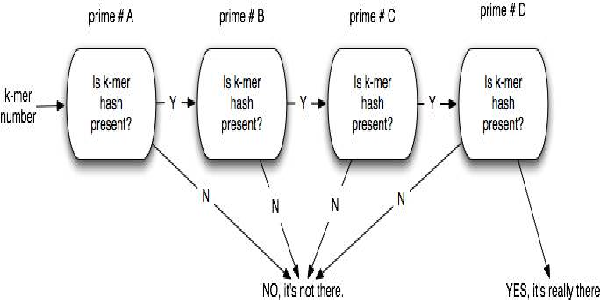
\includegraphics[width=5in]{figures/f1}}
\caption{Bloom filter.}
\end{figure}

\subsection{Effect of false positives}

This representation has a one-sided error that we can measure and
predict in terms of its impact on graph properties.  Link degradation
to percolation here.

\begin{figure}
\center{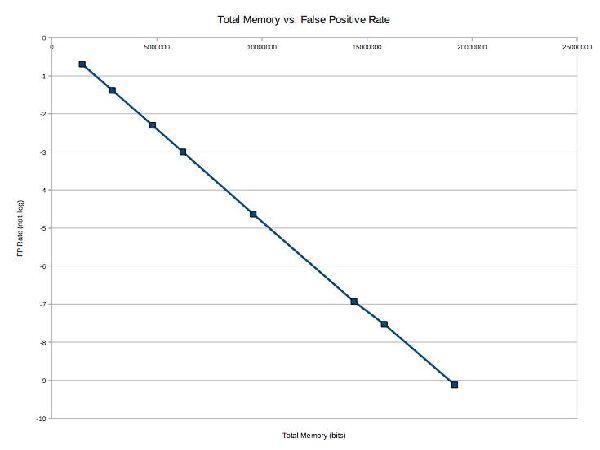
\includegraphics[width=5in]{figures/f2b}}
\caption{Bloom filters scale well.}
\end{figure}

\begin{figure}
\center{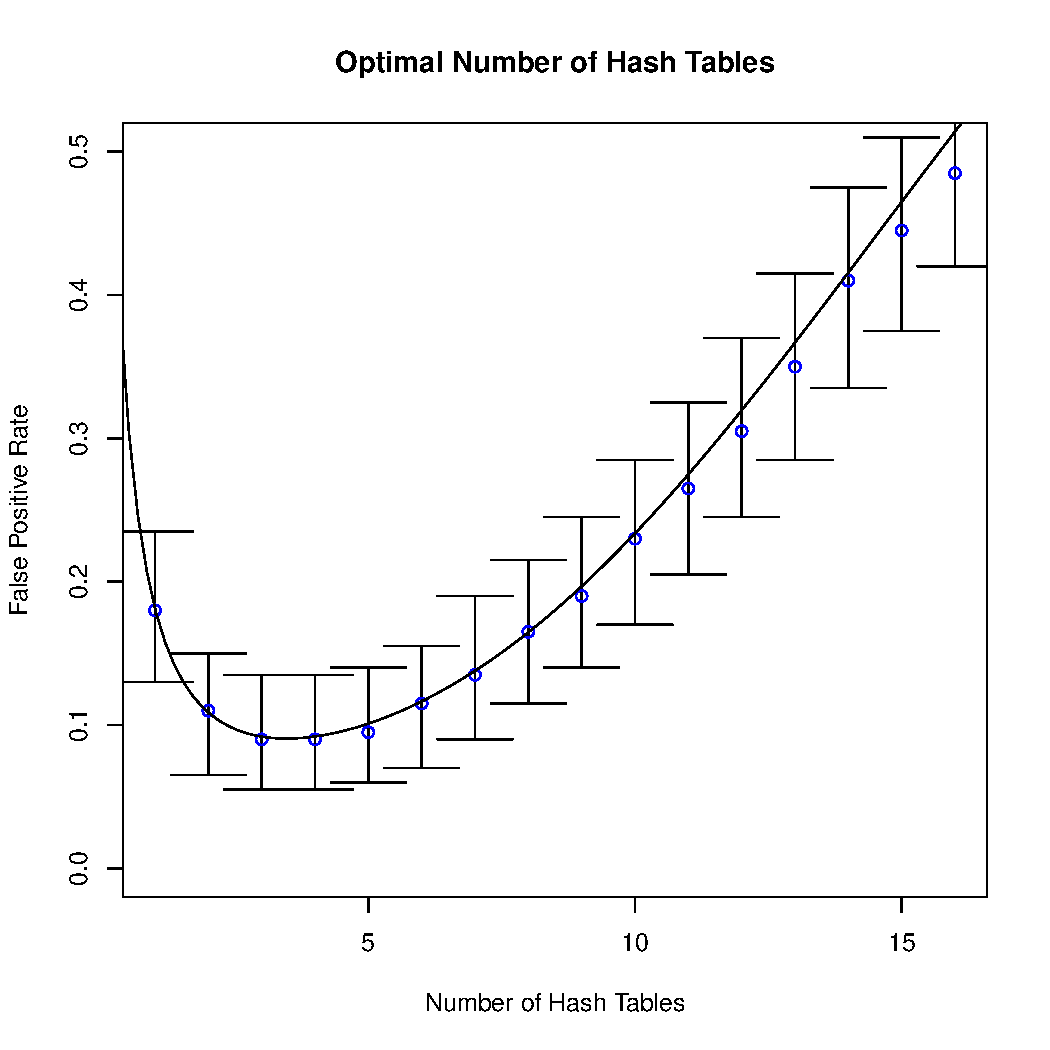
\includegraphics[width=5in]{figures/optht}}
\caption{There is a minimum false positive rate for a given amount of memory
and amount of data, set by the number of hash tables.}
\end{figure}


\begin{figure}
\center{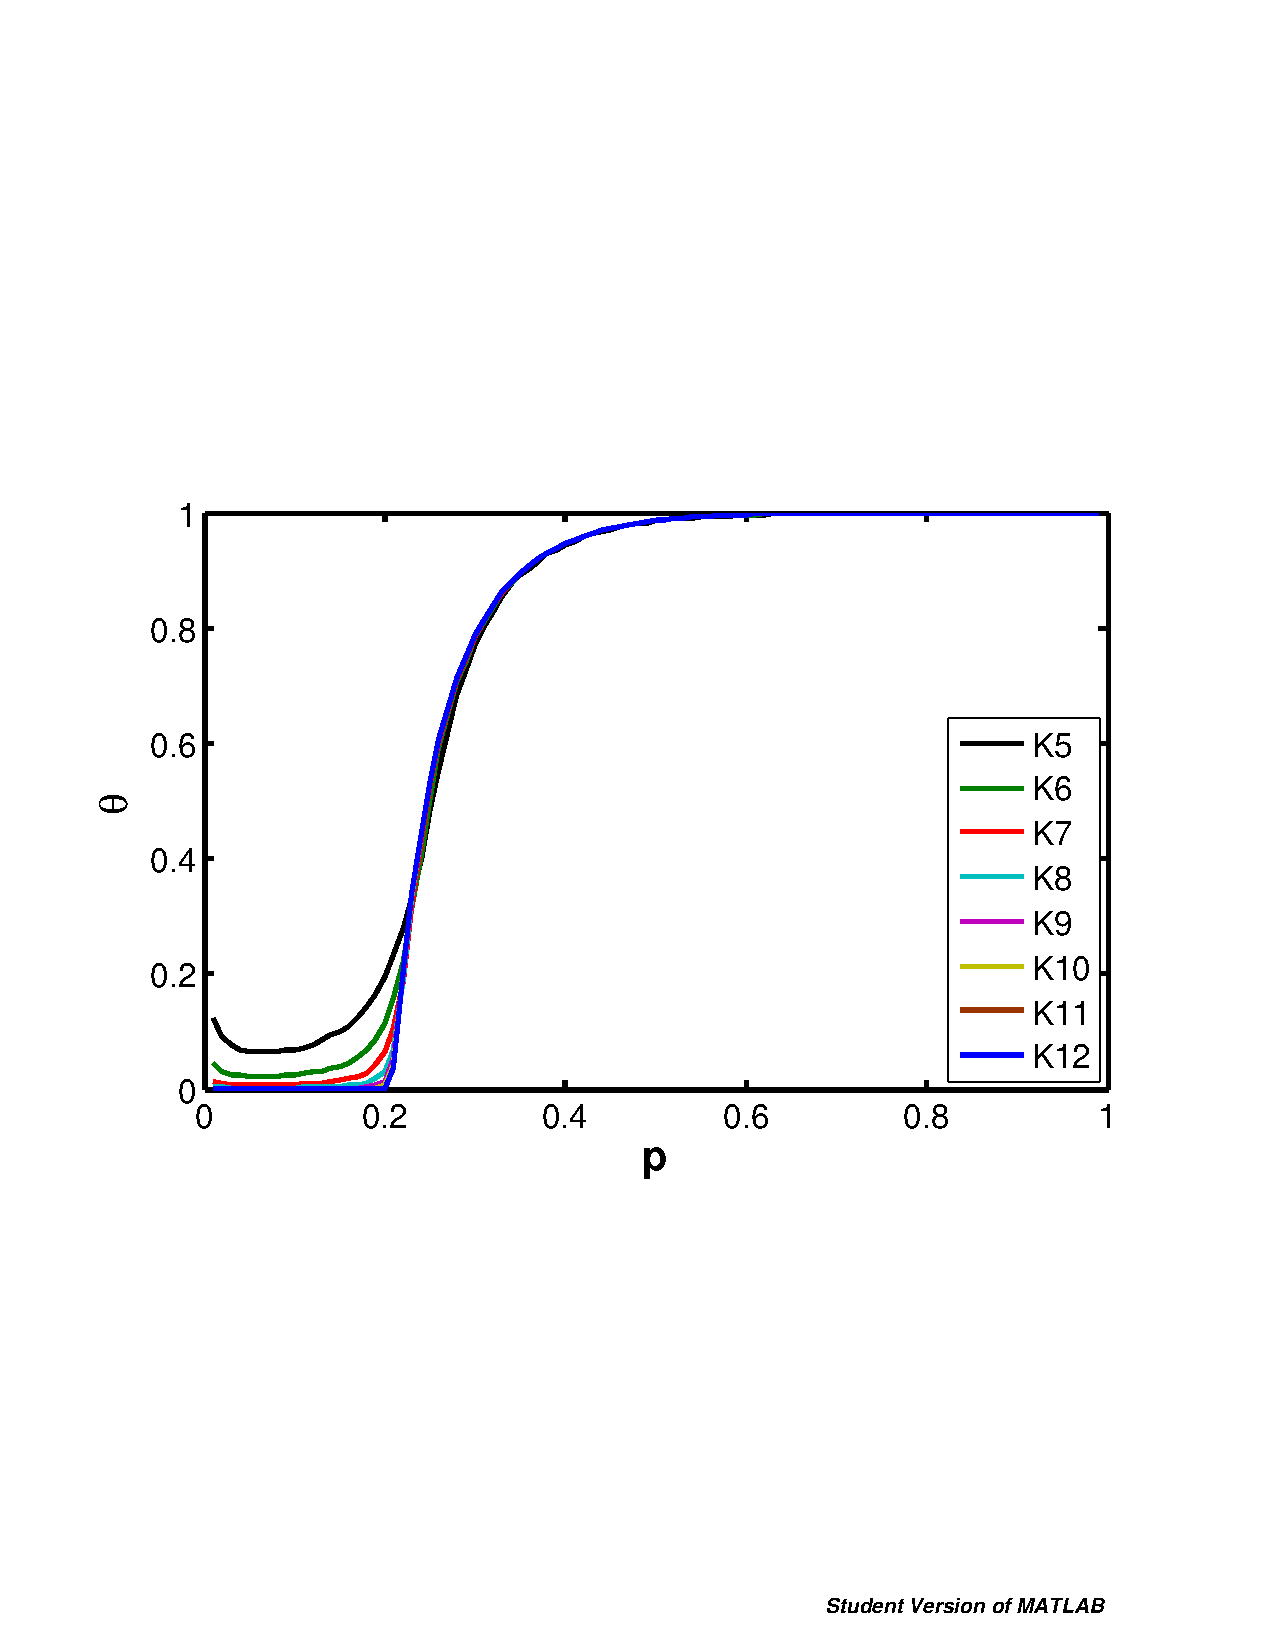
\includegraphics[width=5in]{percolation_K5_to_K12_withLegend}}

\caption{K independence, relative size of the largest connected component
$\theta$ for kMer occupancy p (0.0 to 1.0) of various de Bruijn graphs of
different sizes K (5 to 12 see legend), showing the independence of the
percolation threshold ($\theta = 0.5$) from K.
For each datapoint p 1000 random samples were generated keeping the std error
for each datapoint under 0.0047 while the mean std error for all data points is
$< \approx 0.0002$ (data not shown).}
\end{figure}

\begin{figure}
\center{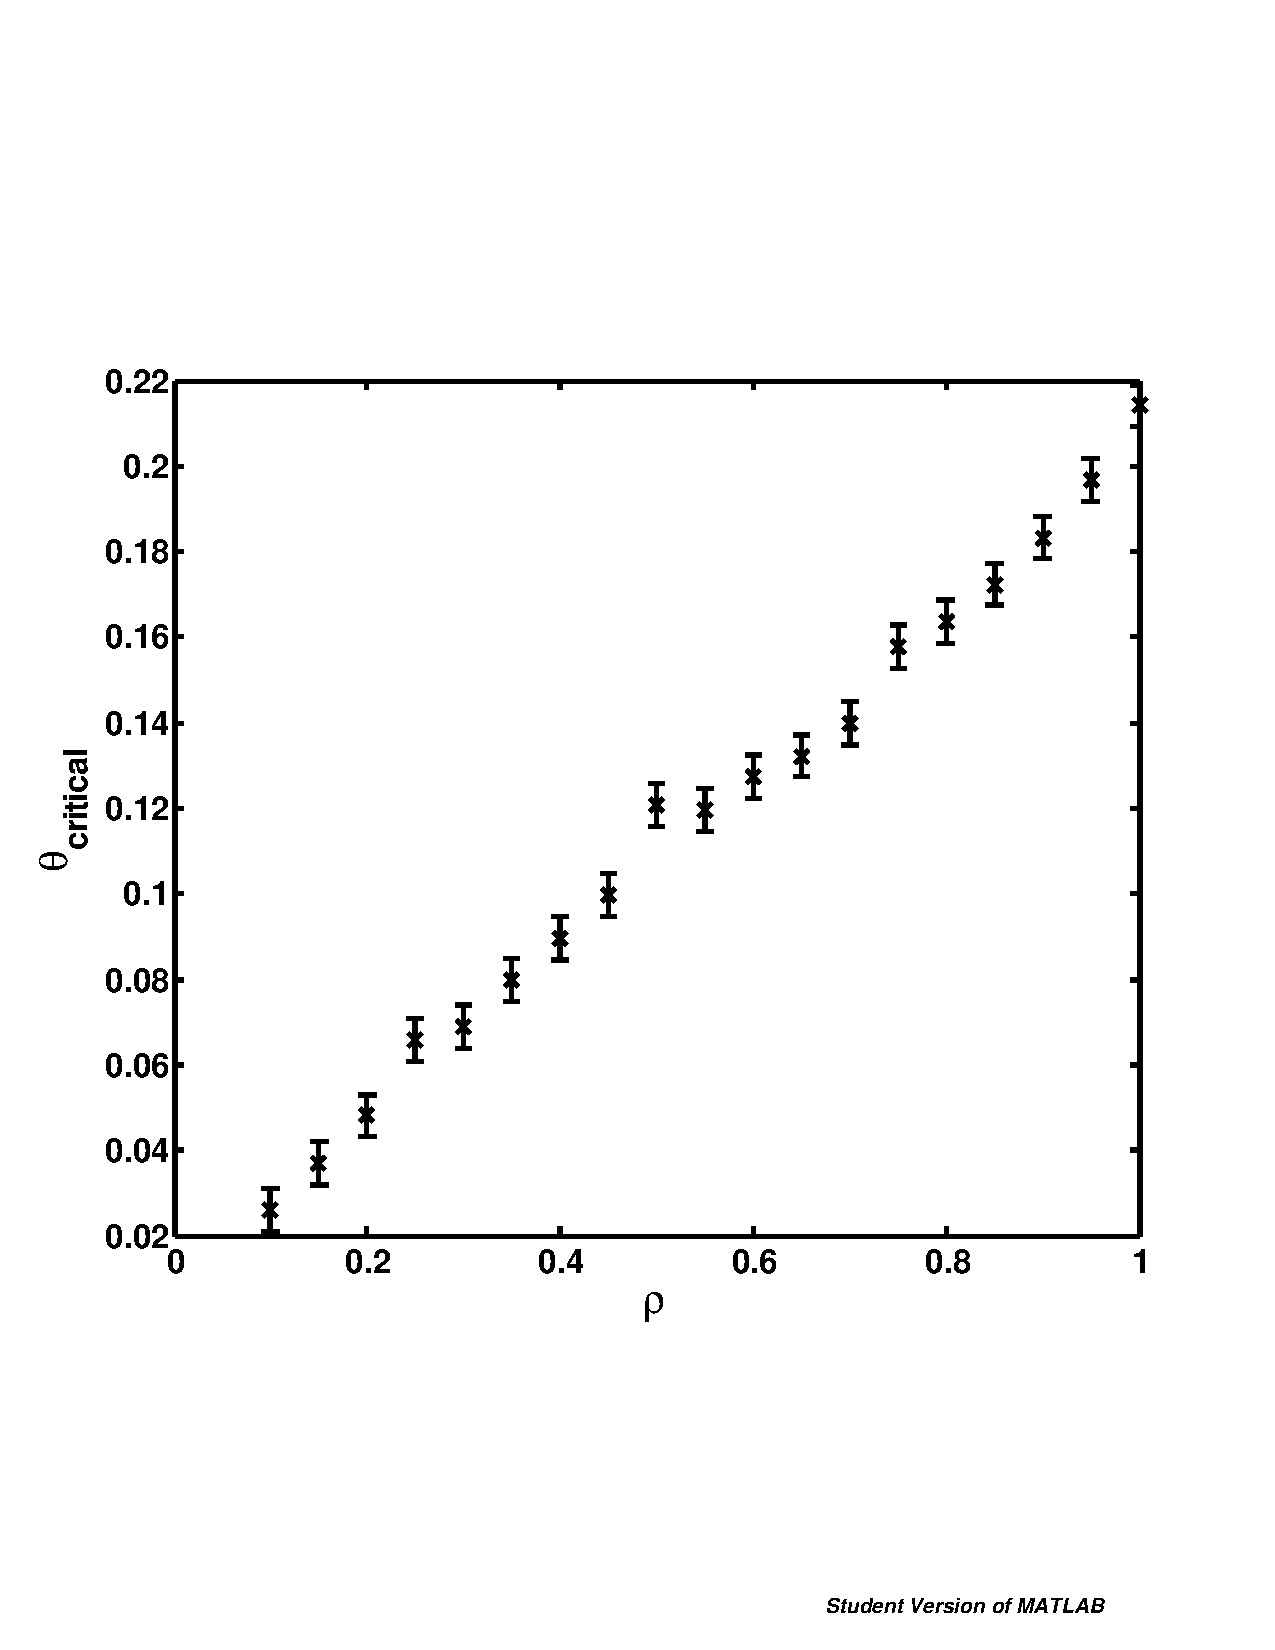
\includegraphics[width=3in]{memoryFraction_vs_percolationThreshold}}
\caption{The critical point for percolation is linearly related to the
  compression factor of the graph representation.
  the following data is wrong...
This figure shows
  the interpolated critical percolation threshold dependence on the
  memory used for the Bloom filter. $\rho$ is the fraction of
  maximally required memory ($4^{12}$ bits) for a de Bruijn graph with
  K=12. We reduced the memory allowed $\rho$ from 1.0 to 0.1 (x
  axis). The critical percolation threshold $\theta_{\rm critical}$
  was linearly interpolated (at the critical point $\theta=0.5$ the
  slope is infinite allowing for this). The std deviation is given for
  each interpolation. This plot shows a linear relation between
  allowed memory and expected percolation threshold assuming random
  data. We can fit the following function to this plot: $\theta_{\rm
    critical} = 0.209 \rho + 0.0052$ describing the fraction of memory
  where random data would percolate.  {\bf CTB: this linear result is
    what you'd expect if the slope of the approach to percolation
    across increased occupancy is exponential, given the logarithimic
    false positive rate wrt memory?}}

\end{figure}

\subsection{This can usefully be applied to assembly graphs}

We can use this to look at local assembly graphs usefully.

\paragraph{Fidelity of local graph properties is tunable.}

\begin{figure}
\center{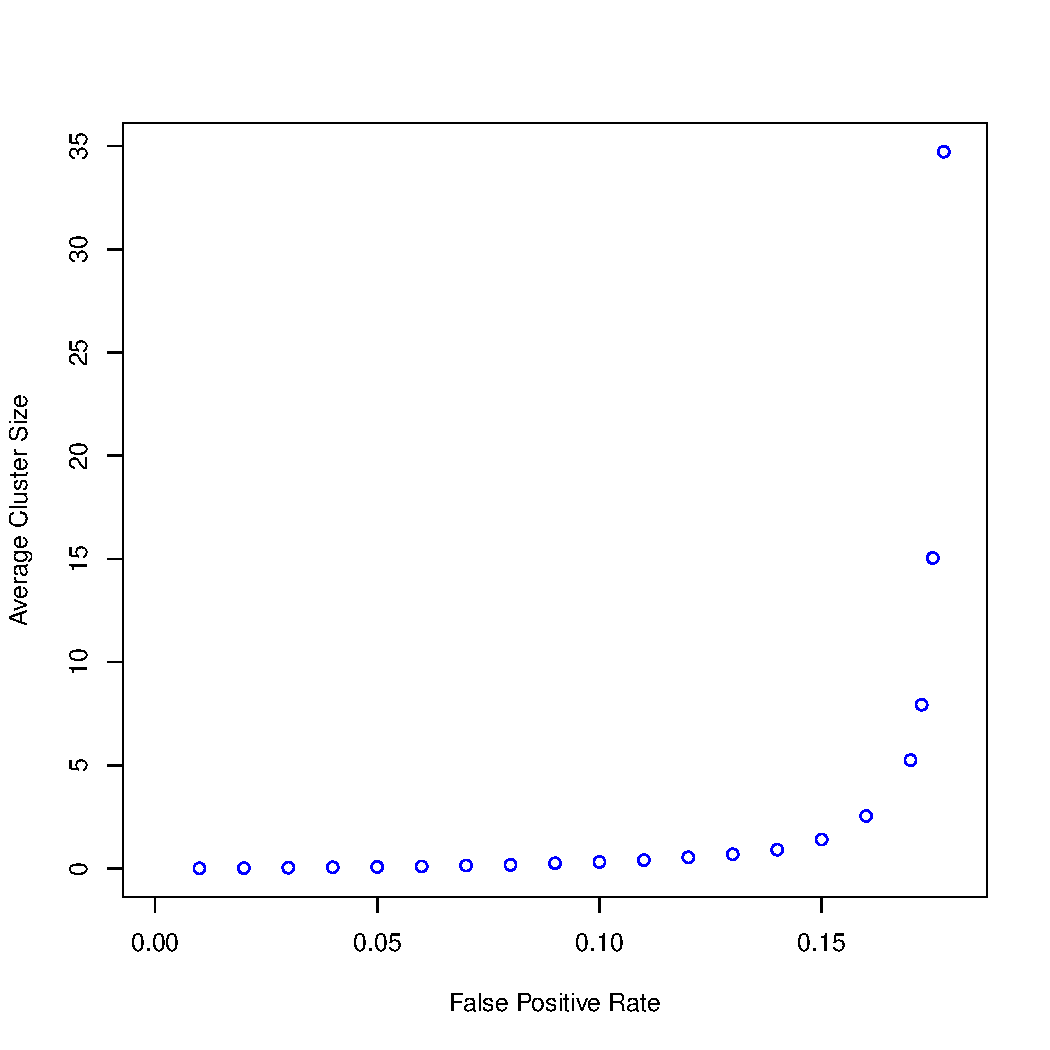
\includegraphics[width=5in]{k31}}
\caption{Approach to critical percolation limit. {\bf Is this an
    exponential?  Or what?  Might be too sharp for that, but what
    would the functional form be? Can we fit?  Do we know the constants?}}
\end{figure}

\paragraph{Large scale graph structure is retained even with high FP rate, out to percolation threshold.}

\begin{figure}
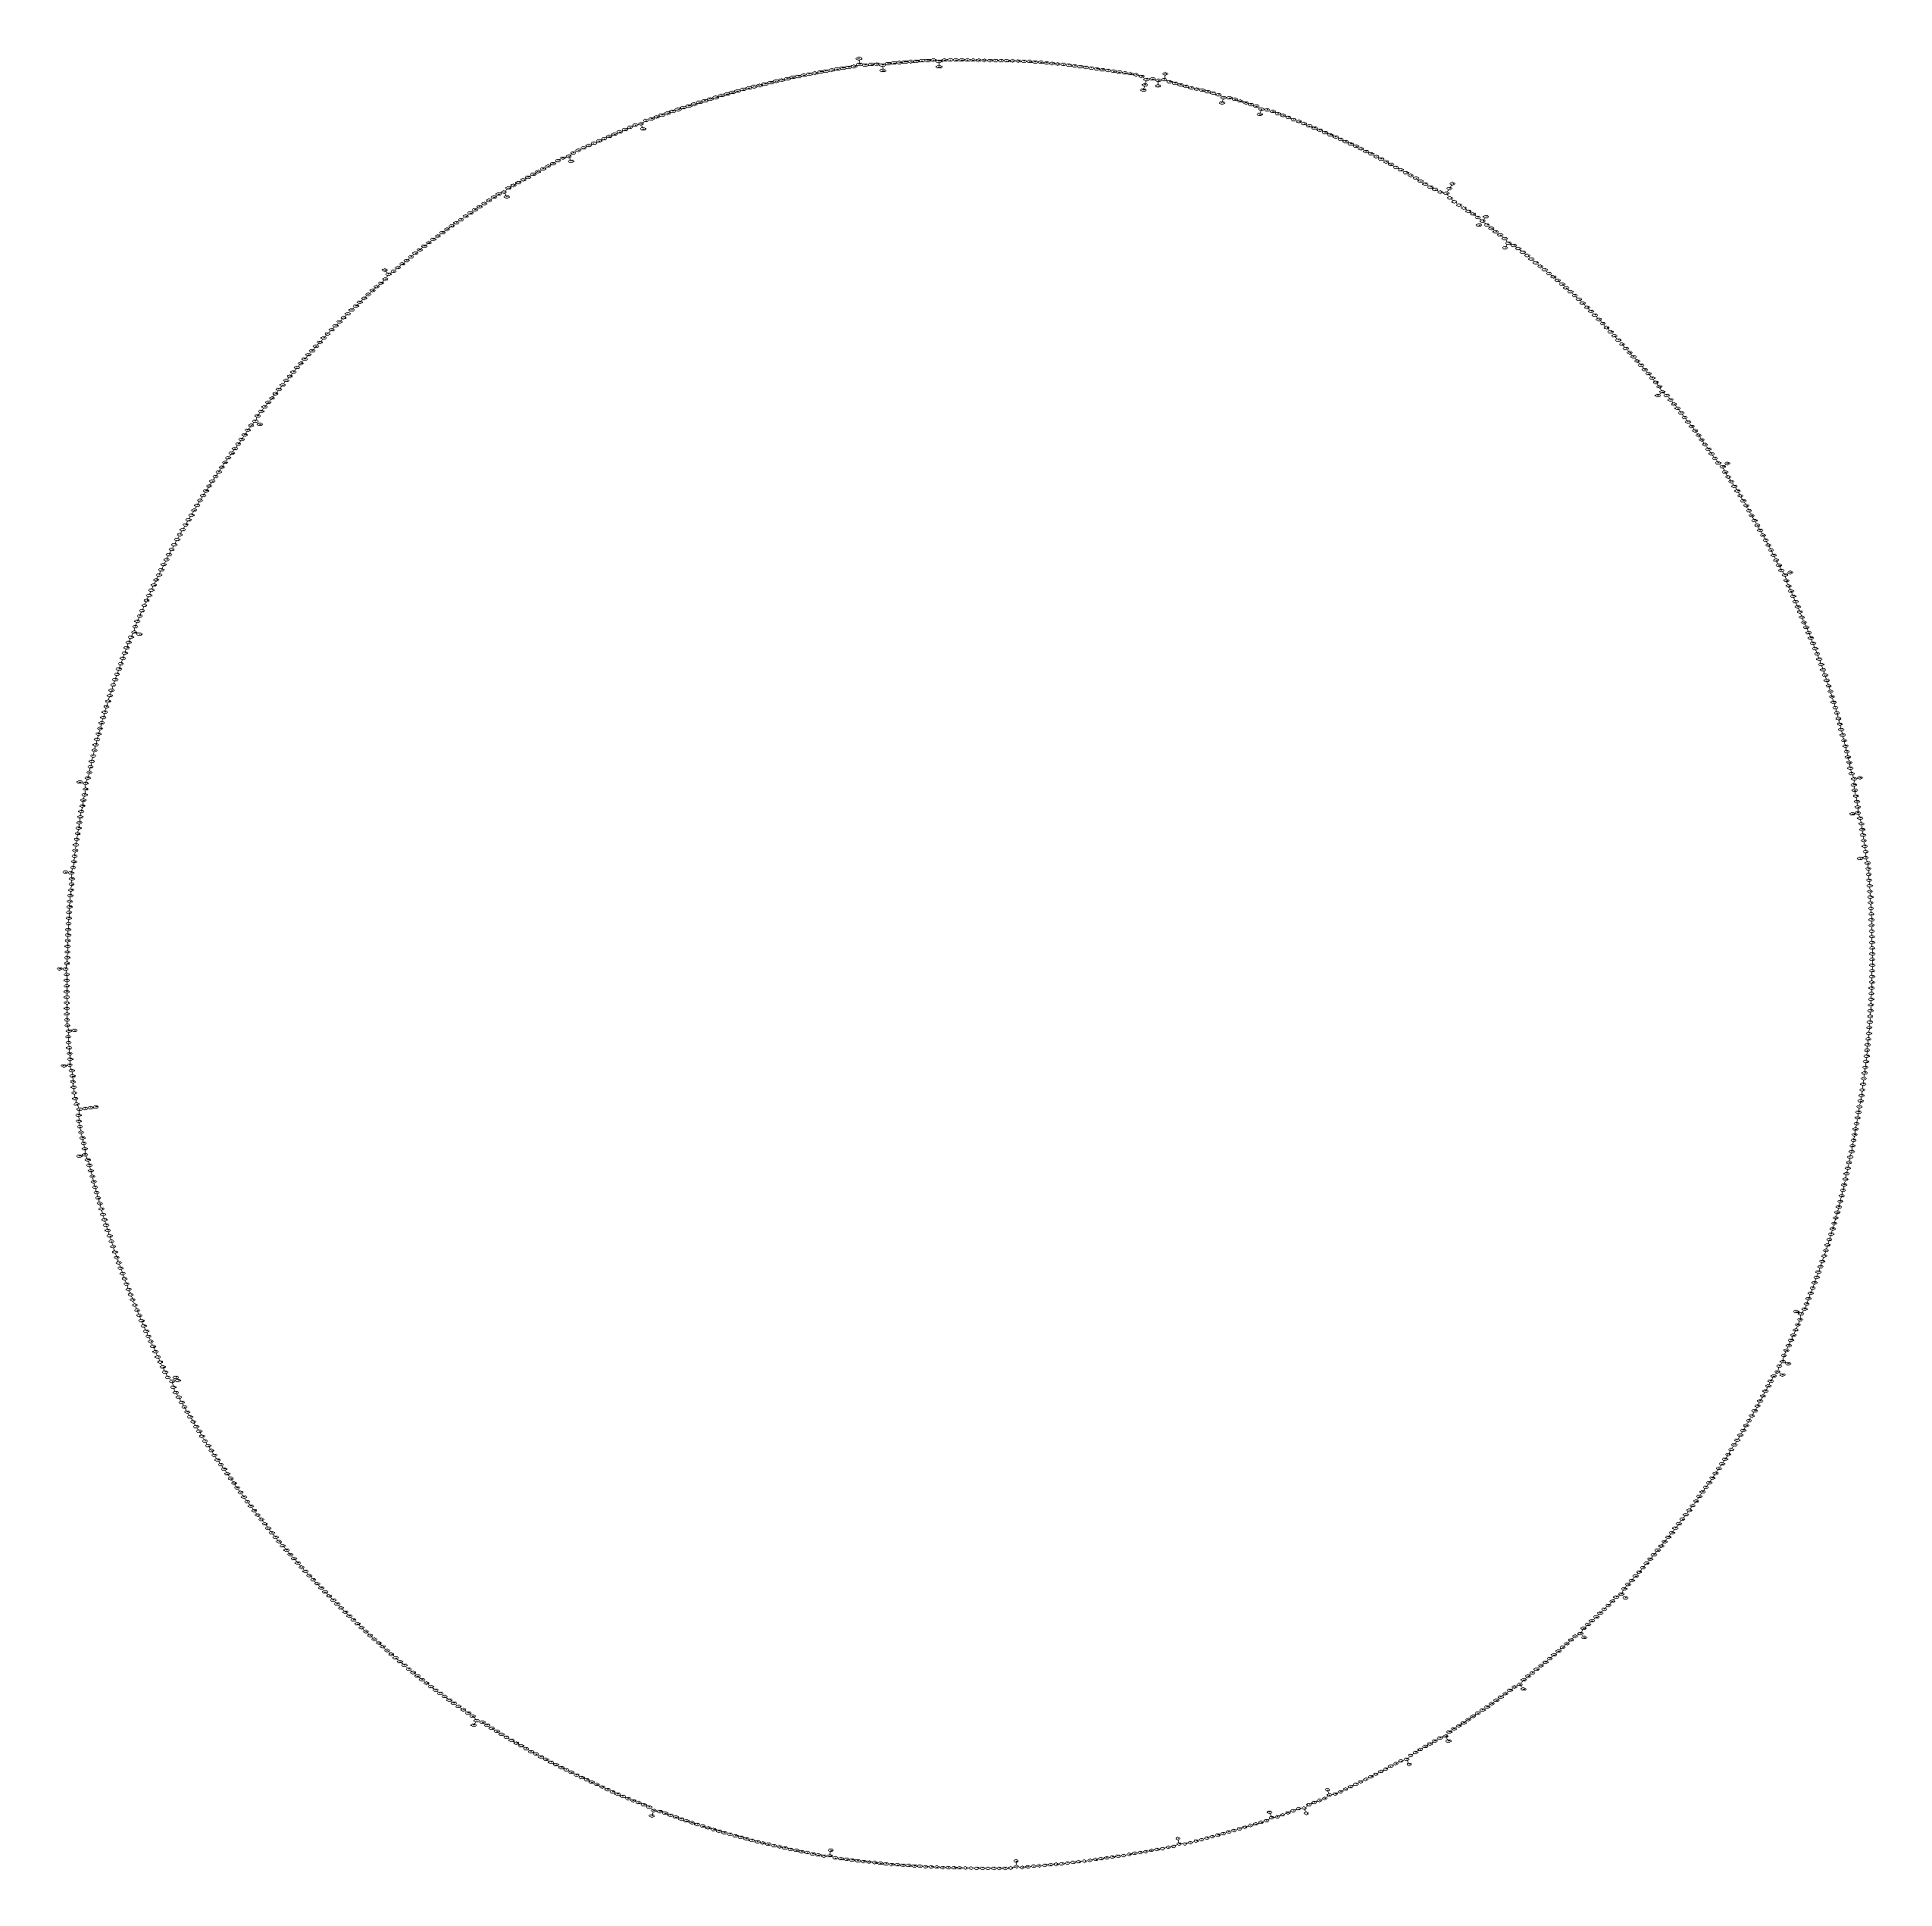
\includegraphics[width=3in]{figures/f3b001}
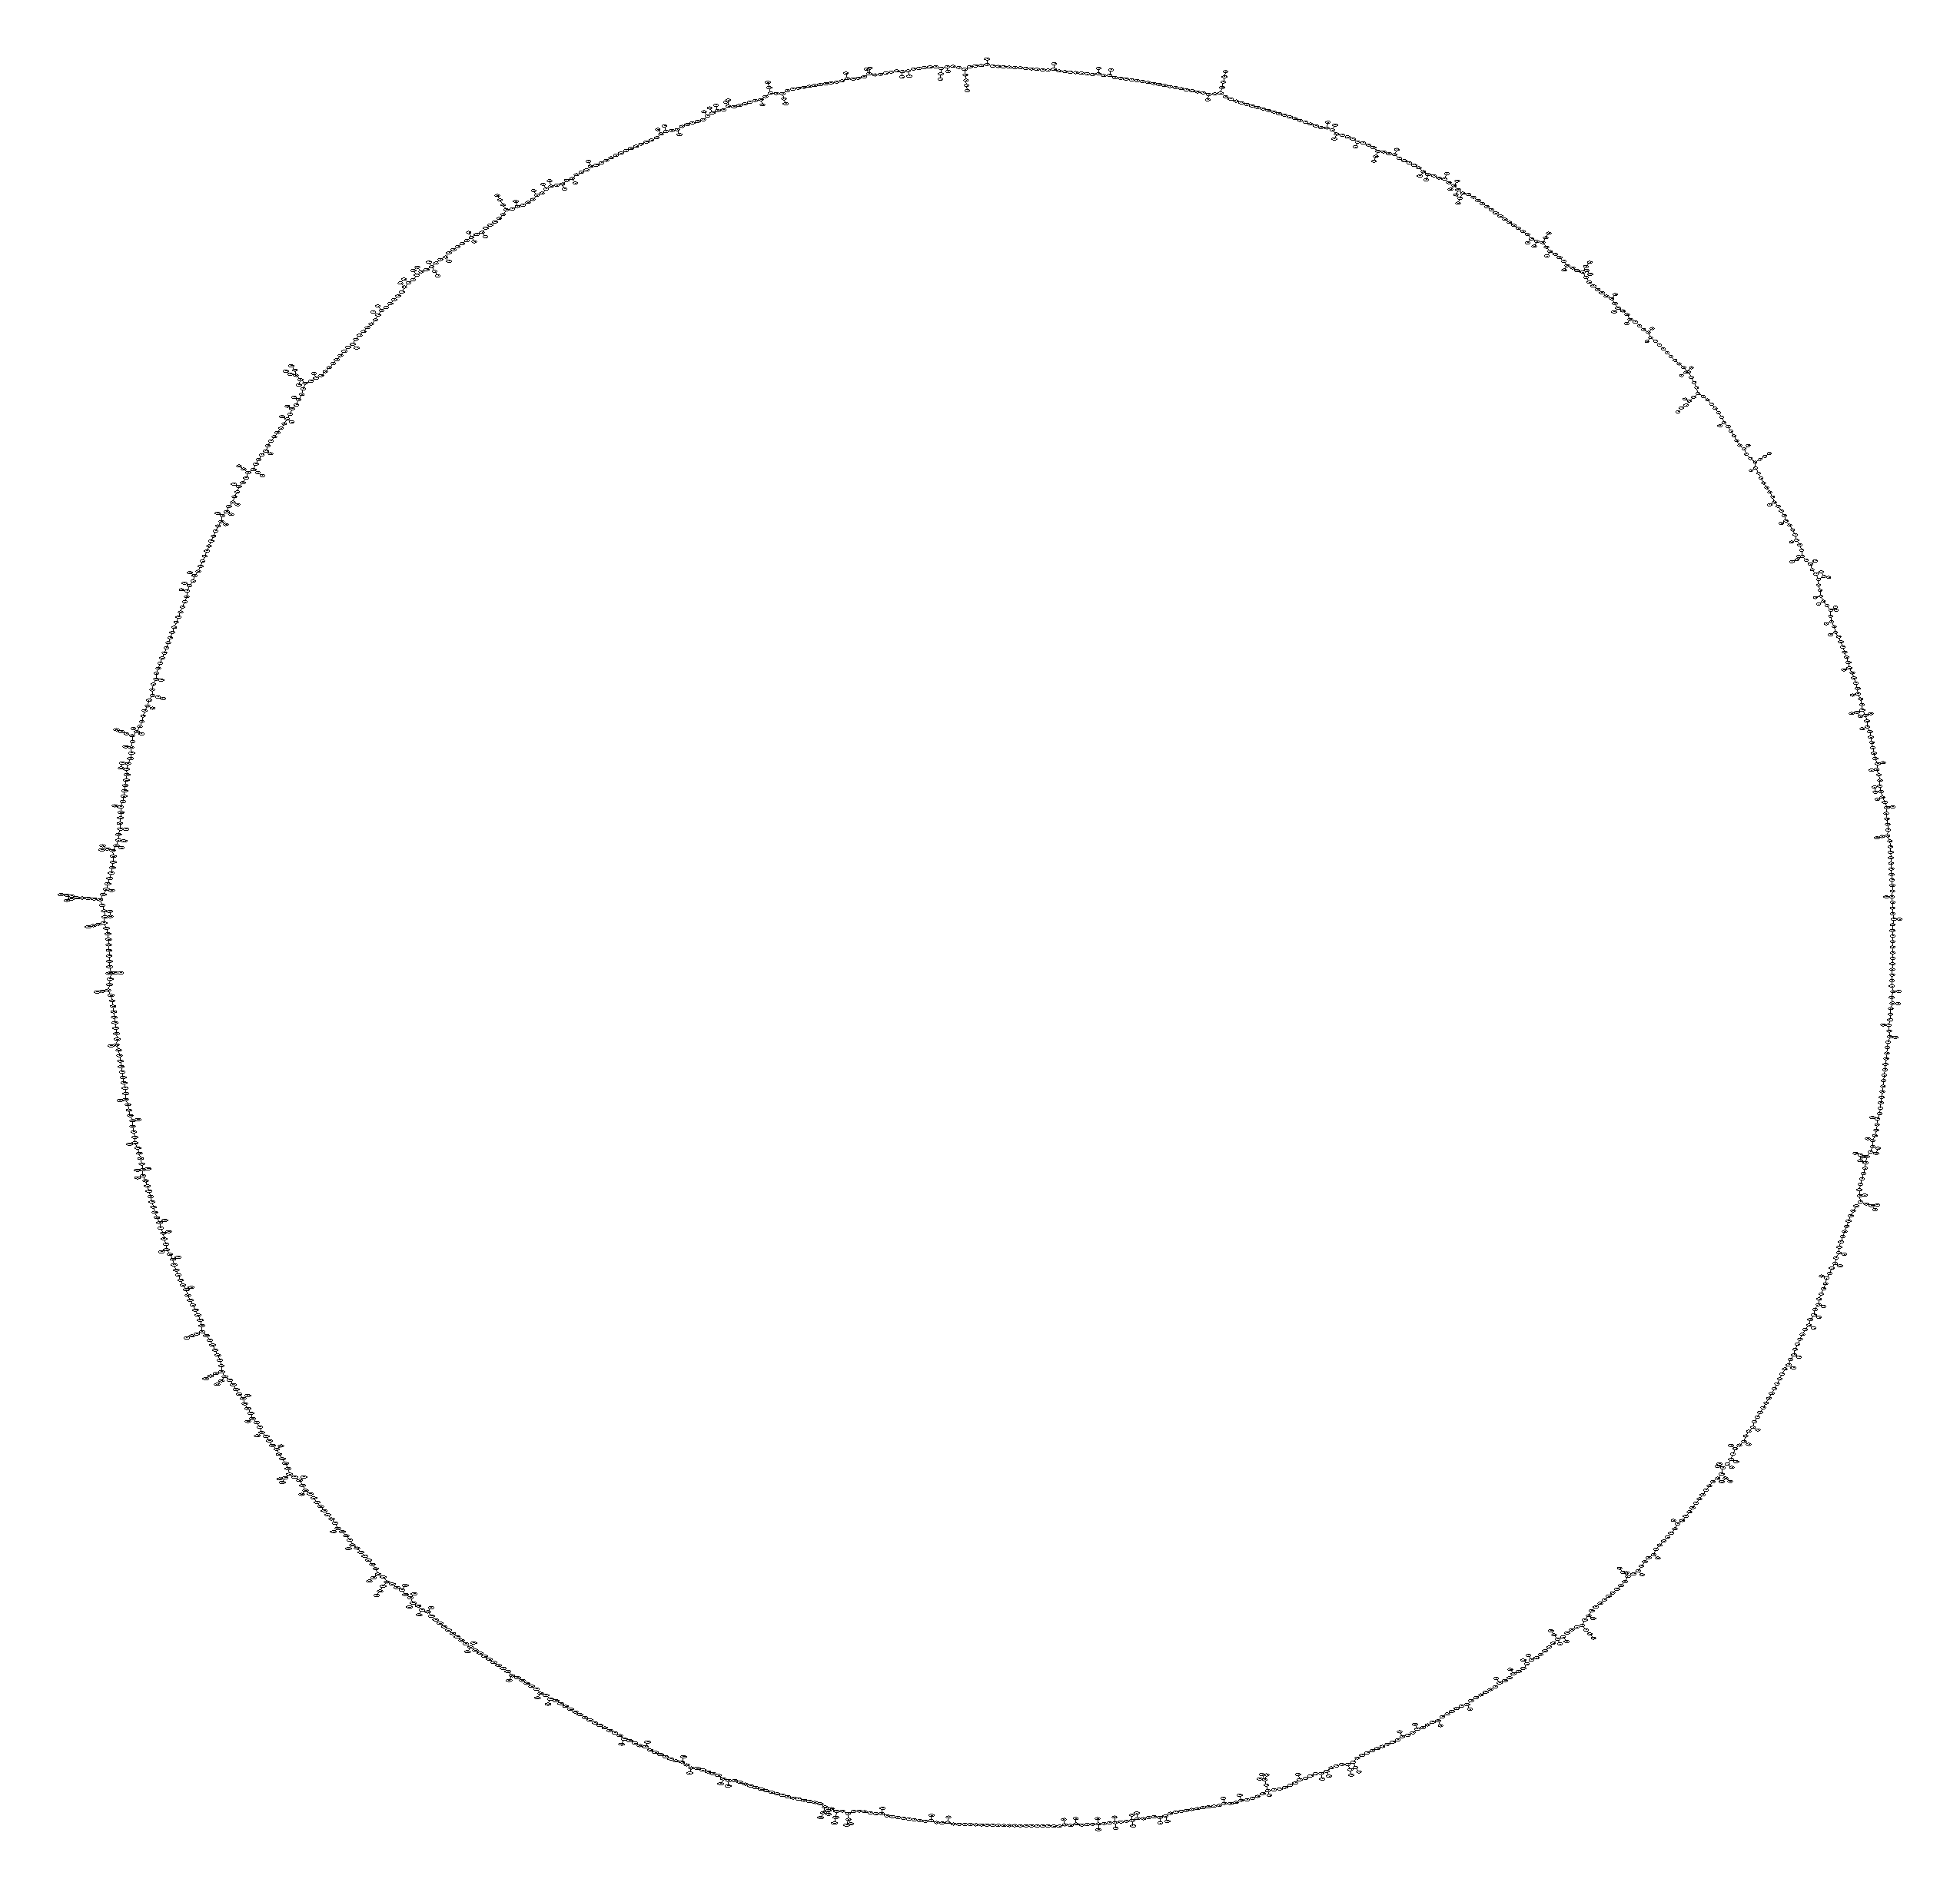
\includegraphics[width=3in]{figures/f3b005}\\
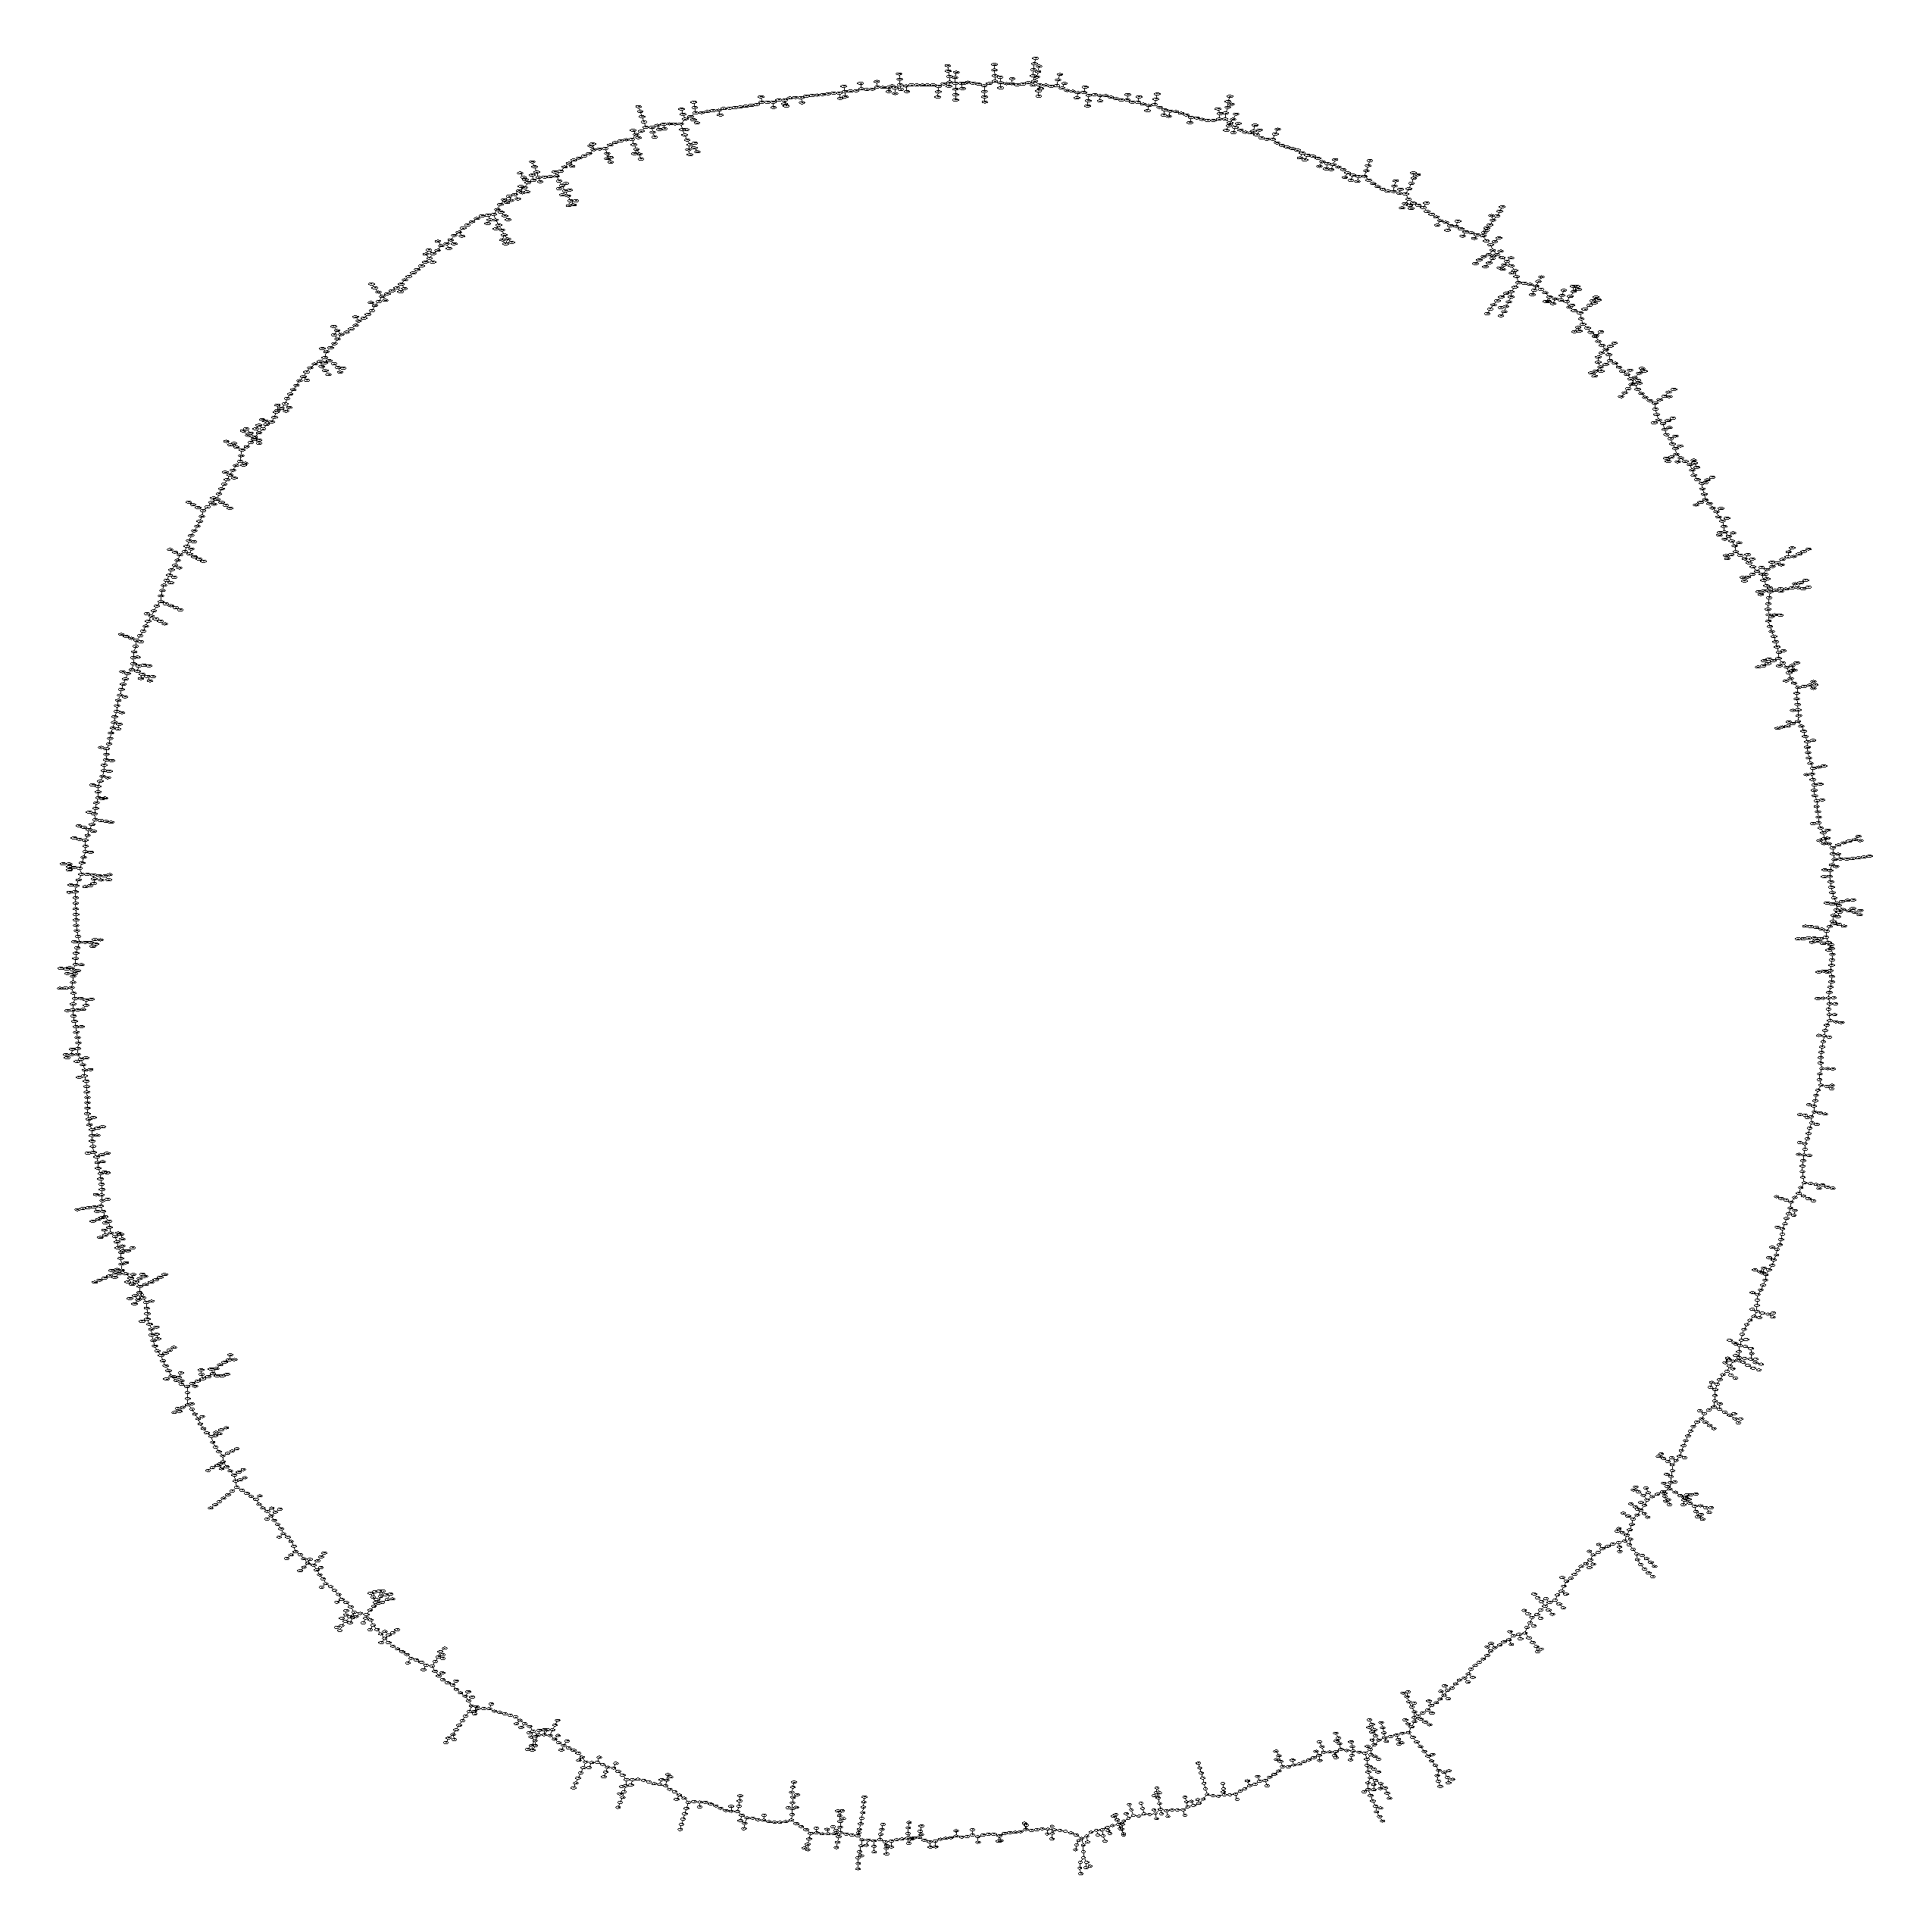
\includegraphics[width=3in]{figures/f3b010}
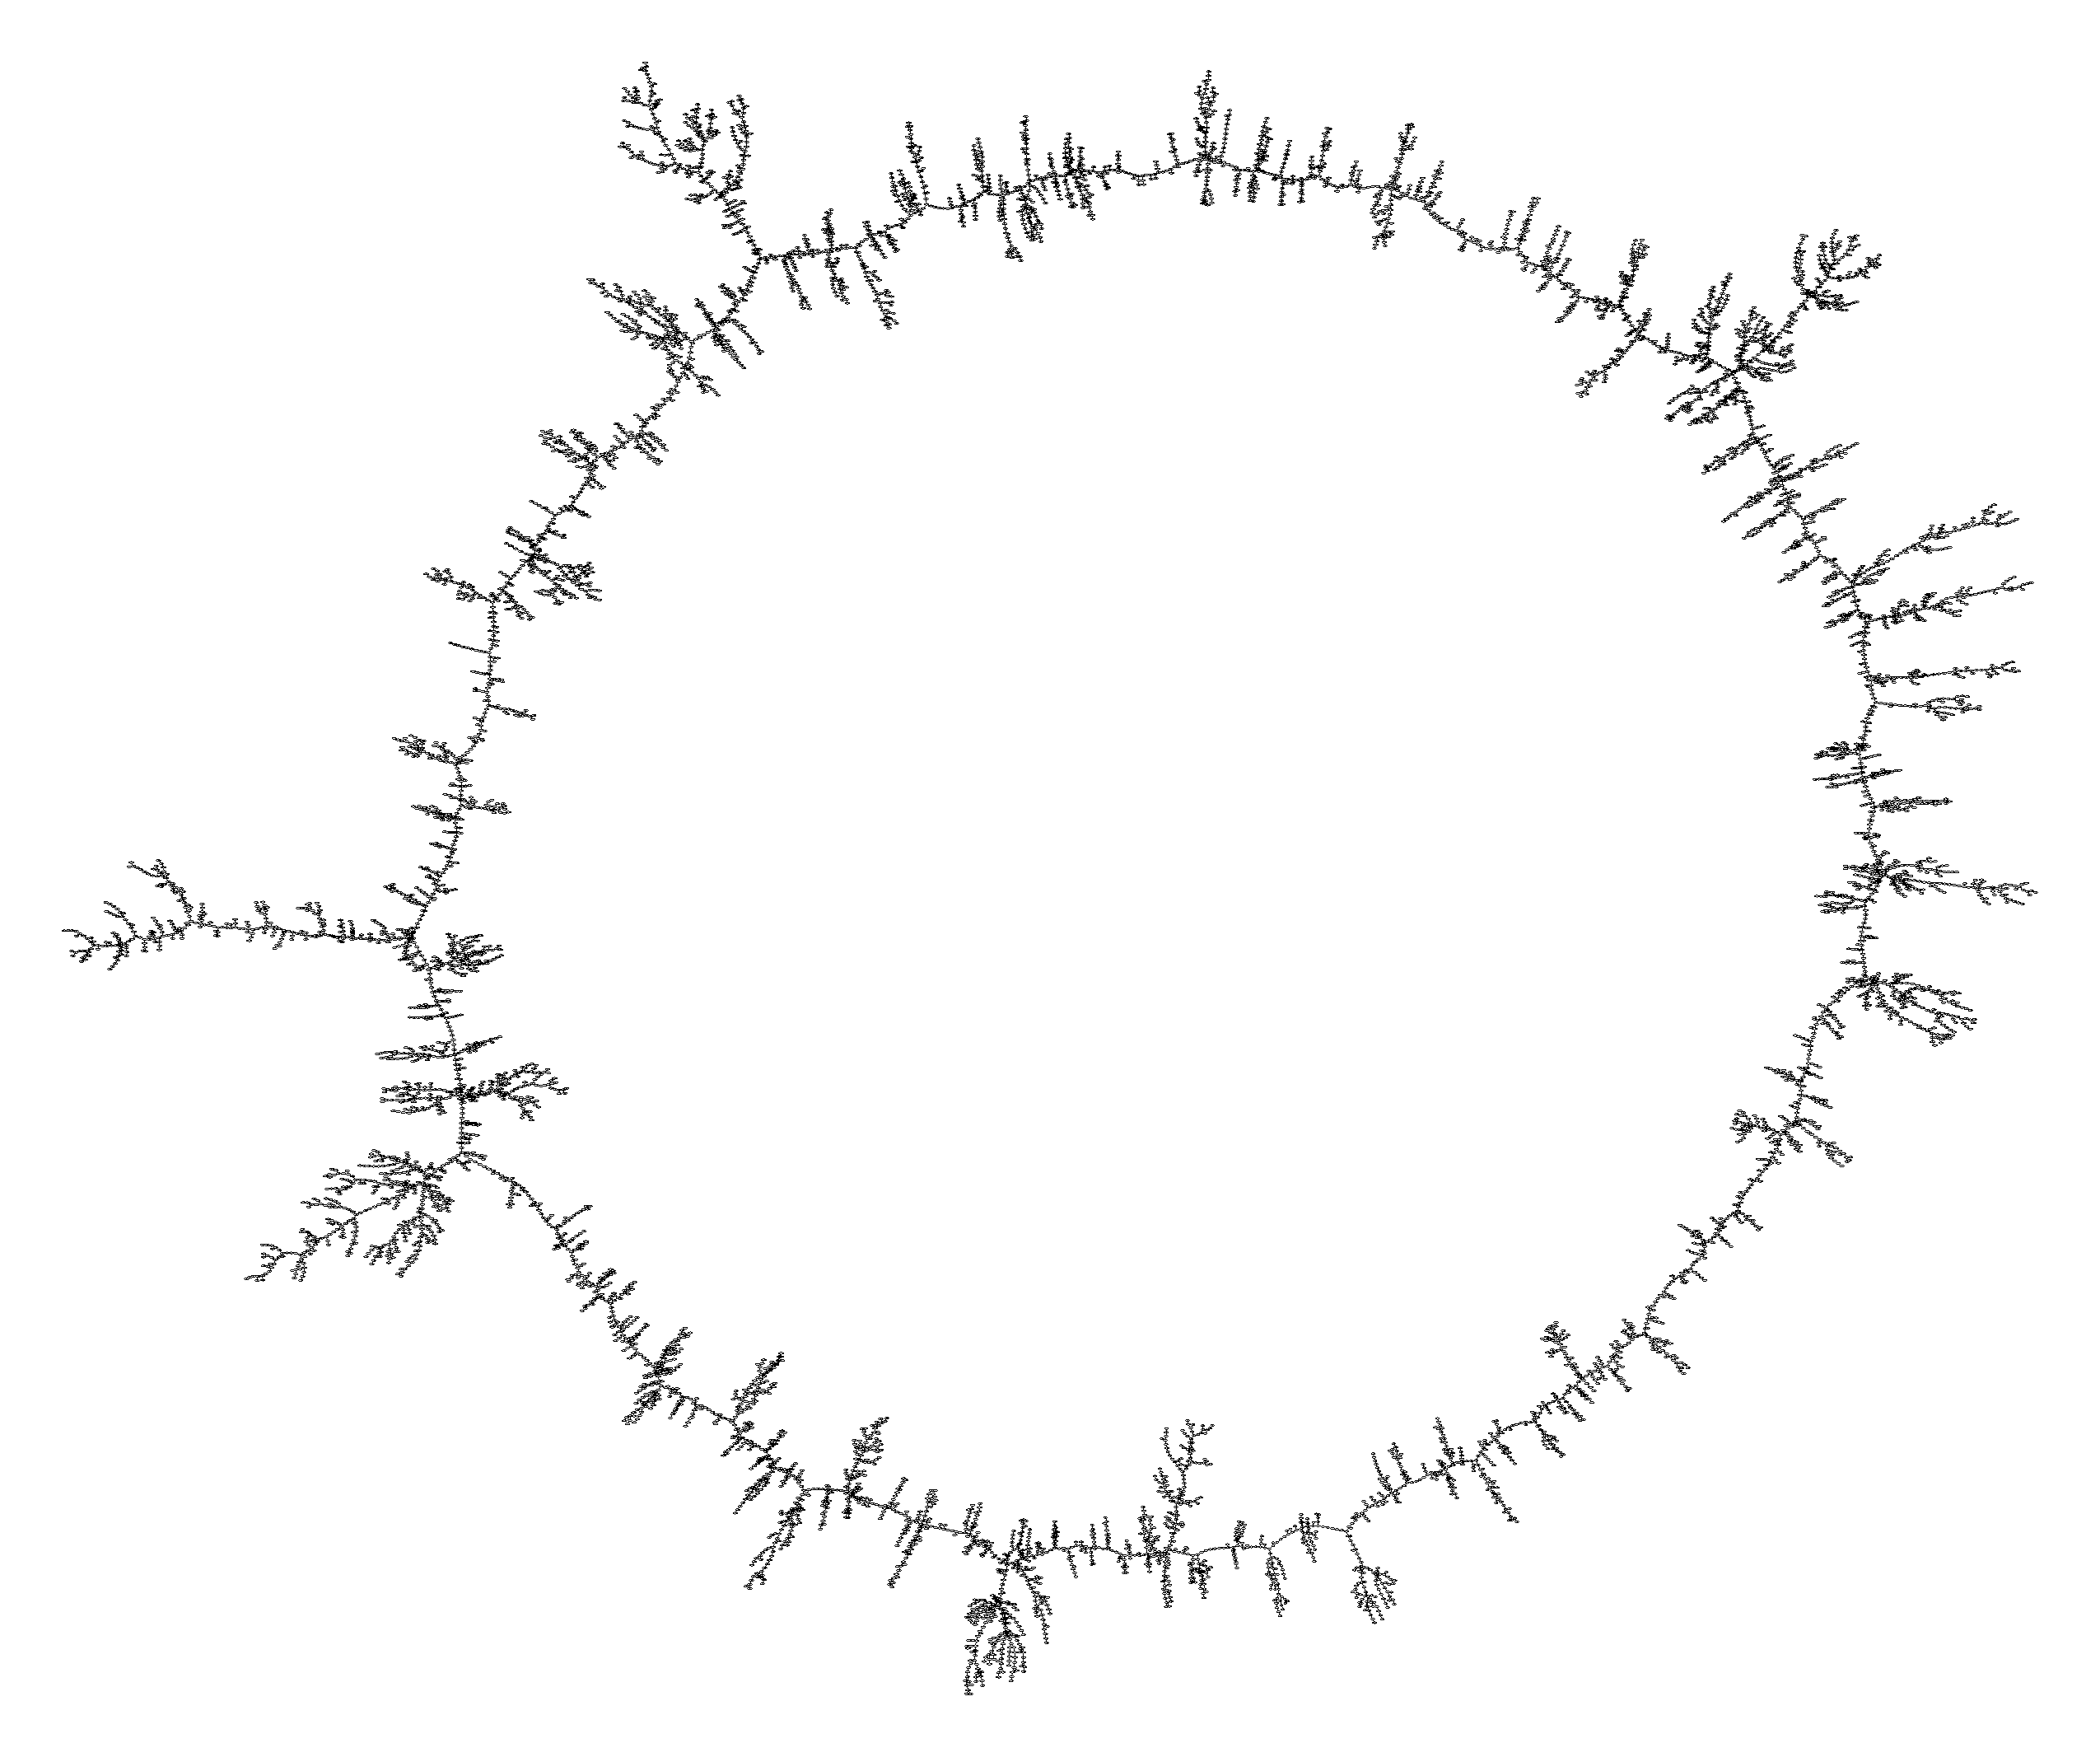
\includegraphics[width=3in]{figures/f3b015}
\caption{Decreasing fidelity of graph structure with false positive rate.
{\bf CTB: This should be out first figure, I think!}}
\end{figure}



\paragraph{Both local and large scale graph structure fidelity is preserved for relatively low memory representations.}

\paragraph{We can partition exact data and inexact (error-prone) data.}

\begin{figure}
\center{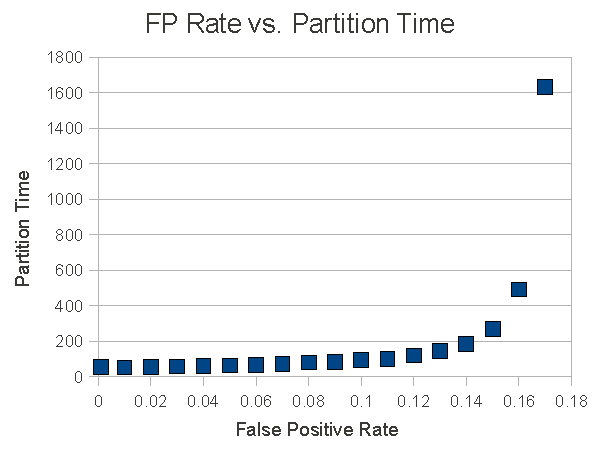
\includegraphics[width=5in]{figures/f3d}}
\caption{Computation required to partition graphs grows with false positive
rate.  CTB: good to know, but I think this figure can go away; it's implied
by everything else.}
\end{figure}

\paragraph{Link error-prone sequencing to percolation threshold?  Error inflates number of unique k-mers being added in => increases memory requirements.}

Can we discuss sequencing errors for PacBio and link to percolation (show
that even reasonably high sequencing error rate would not percolate?)

100x coverage issue.

\begin{figure}
\center{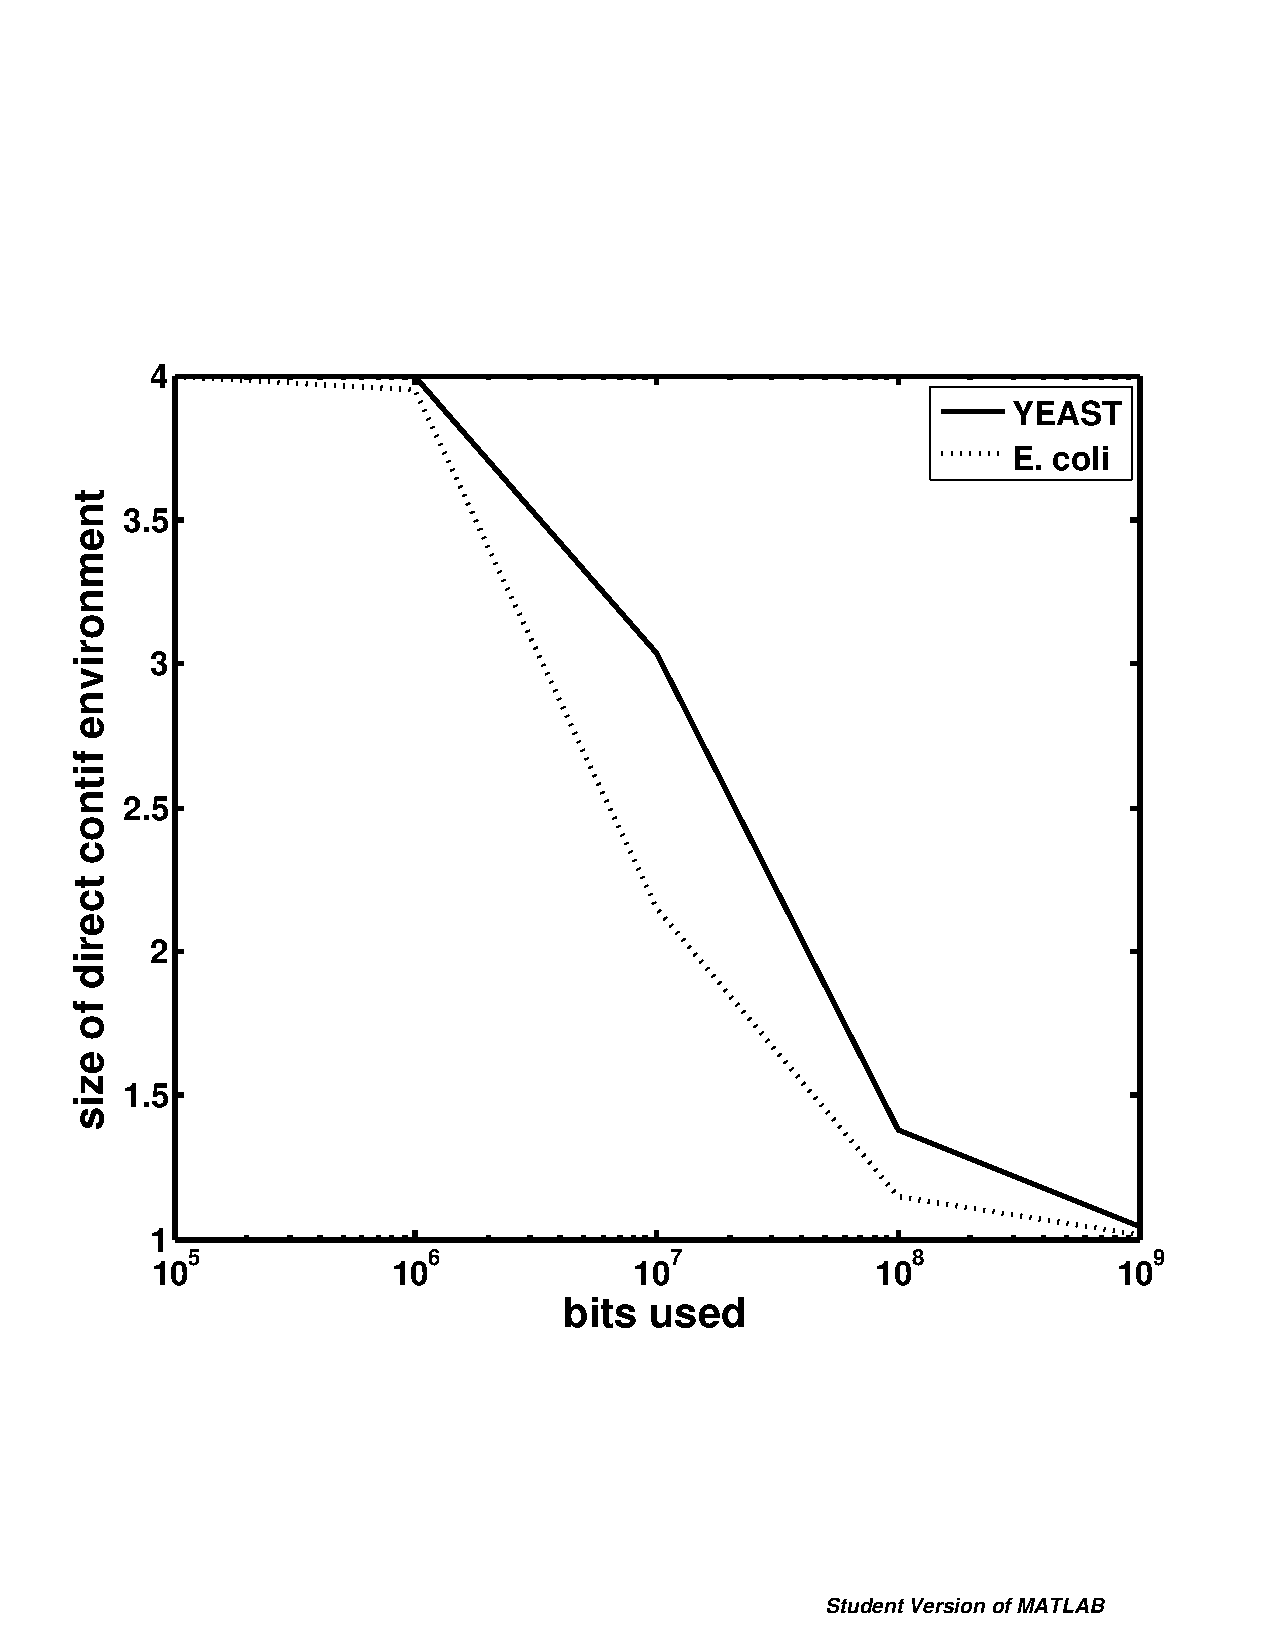
\includegraphics[width=5in]{contigEnvironment}}
\caption{Number of false connections introduced by inexact k-mer storage.
k = ??}
\end{figure}

\begin{figure}
\center{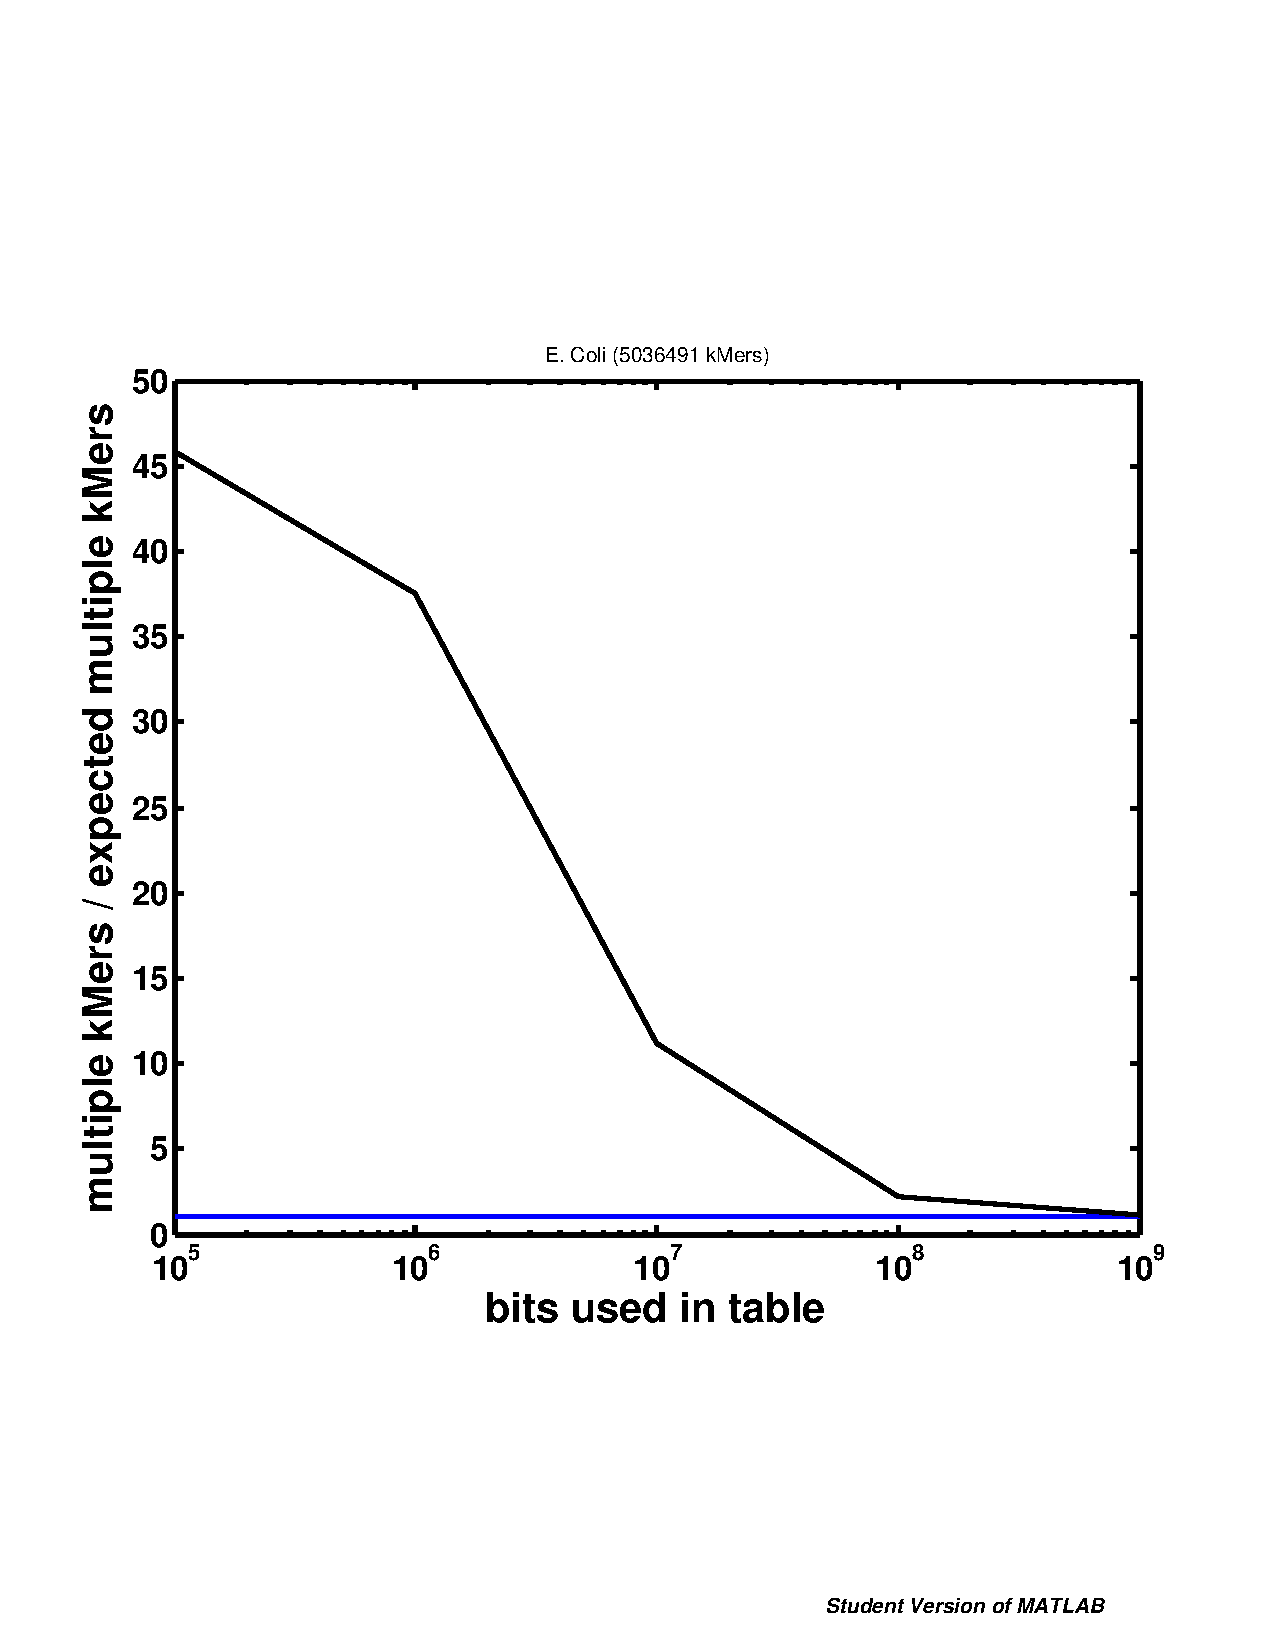
\includegraphics[width=5in]{fractionOfFoundDoubleHitsECOLI}}
\caption{The difference between exact and inexact kmer storage for the
ecoli genome. k = ??}
\end{figure}

\begin{figure}
\center{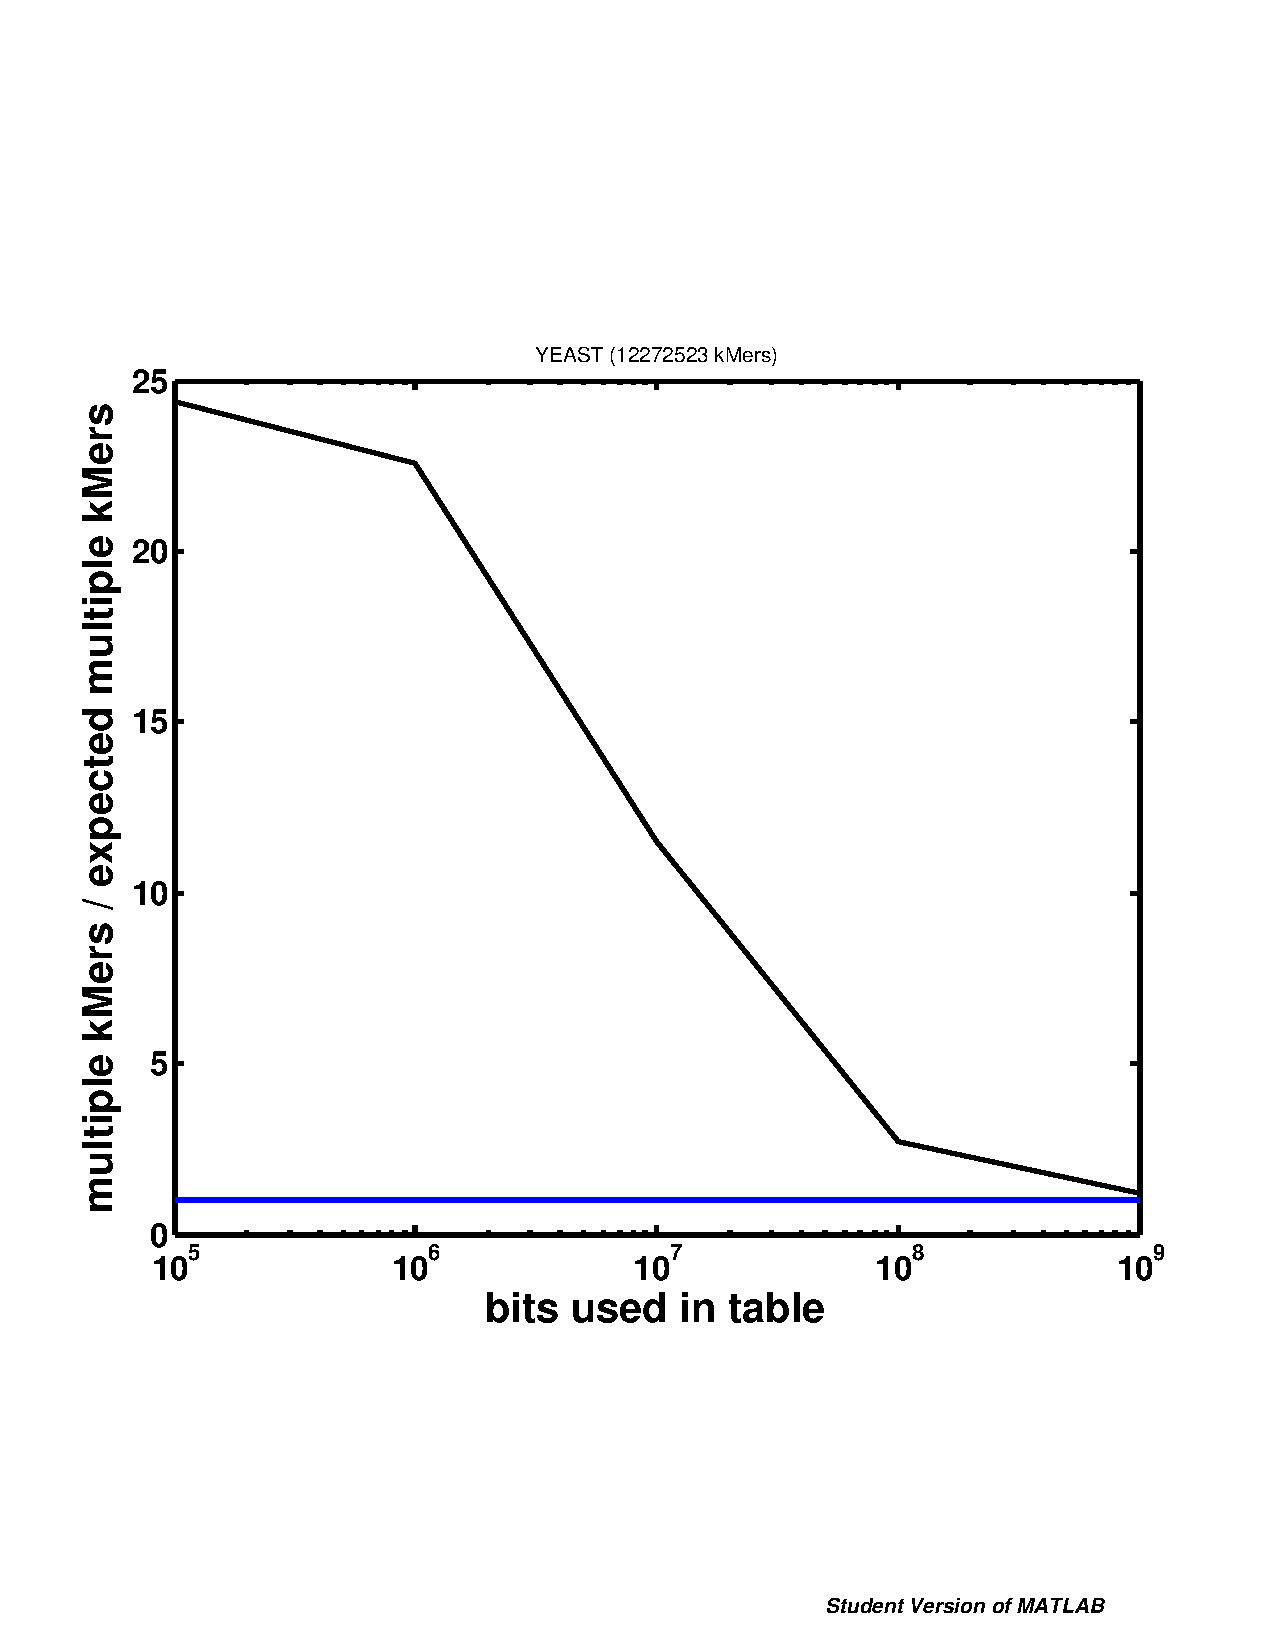
\includegraphics[width=5in]{fractionOfFoundDoubleHitsYEAST}}
\caption{The difference between exact and inexact kmer storage for the
yeast genome. k = ??}
\end{figure}

Idea for last graph:

We would do an exact representation of the E.coli genome, an exact 
representation of an Illumina dataset for E.coli, and then inexact
representations for each with different false positive rates (1\% and
10\%). We can then compare the exact genome versus other types to see
how the number of unique kmers, the number of duplicate kmers, and the
average neighbors per vertex changes. Ultimately, we would be able to
argue that the number of erroneous k-mers created by Illumina
sequencing eclipses that of what is created using our approach.

\section{Discussion}

\subsection{Bloom filters can be used to accurately store large assembly
graphs}

The compressible graph representation we have built on a Bloom filter
is an efficient way to store and traverse k-mer graphs.  Per k-mer
memory usage is low, and independent of k, while k-mer node lookup and
local traversal are constant time.  The primary data structure can
also be implemented in constant memory.  This graph representation is
also extremely simple to implement and verify.

The probabilistic nature of the data structure is a significant
concern, but the collision rate and resulting increase in false local
connectivity are very predictable.  On a larger scale, we can link the
rate of increase in global connectivity from false positives to a
first-order phase transition, which lets us define a broad range of
parameters for which global graph structure is extremely accurate.

The effect of increasing false positive rate as ``error'' can be
compared to the effect of sequencing errors.  Sequencing error
introduces both false negatives (by eliminating ``true'' k-mers from
low coverage samples) and false positives.  False positives and
negatives from sequencing errors also often result in k-mers that are
a low Hamming distance from the true k-mer, which can result in
elaborate graph structures.  In contrast, the Bloom graph error is
entirely one-sided, only resulting in false positives; moreover, these
false positives are uncorrelated to the ``true'' k-mers from which
they arise, and do not generally contribute to local graph structure.

Overall, the Bloom k-mer graph is an efficient data structure for
storing and traversing large k-mer graphs.

\subsection{Using Bloom k-mer graphs for DNA sequence assembly}

Bloom k-mer graphs may not be directly useful for traditional
approaches to DNA assembly, which rely on systematic heuristic
transformations of graph structure to find an optimal path through the
graph.  This is because the Bloom graph, as presented here, is limited
to representing k-mer graphs for a fixed k, and paths cannot readily
be compacted or eliminated.

There are many uses, however, for an extremely scalable
constant-memory graph representation.  Below we discuss the use of the
Bloom k-mer graph data structure as a lens for exploring graph
properties and filtering data sets.

For low-coverage samples, assembly graphs may contain many small
unconnected components, that represent unconnected sequences.
Sequences contributing to these unconnected components can be safely
eliminated from the originating data sets without affecting the final
assembly.  This can be done efficiently with a simple limited depth
graph search algorithm.

More generally, assembly graphs may contain many disconnected
subgraphs, due to the structure of the source data (e.g. transcriptome
or population sequencing) or because of low coverage.  These subgraphs
can safely be partitioned into different graphs without affecting the
final assembly, reducing the memory and computation required for
assembly of the whole to that required for the largest subgraph.
(@@ Discuss iteration here as a way to get rid of false positives.)

The Bloom k-mer graph can also be used to do de novo repeat discovery
in collections of unassembled reads.  This in turn can be applied to
filtering of repeats prior to assembly (ref Hydyra), or for isolating
repeats from shallow or exploratory sequencing efforts.

It should also be possible to adapt sequence structure (e.g. ORF),
homology (BLAST), and domain search (HMMER) algorithms to search this
graph structure instead of searching either unassembled reads or
assemblies.  Because assembly graphs implicitly collapse identical
sequences into a single path, this may be a more scalable approach to
targetted-gene analysis for metagenomics than current approaches
(which rely on searching individual reads).  Also note that, unlike
sequencing errors, the false positives in the Bloom graph will
generally bear no resemblance to biologically valid matches.

The Bloom k-mer graph could also be used to develop connectivity-based
read trimming and correction algorithms.  For example, low-abundance
reads that contribute to ``spurs'' or ``sidings'' in otherwise
high-coverage regions could be corrected to match the
consensus, or trimmed to eliminate the divergent sequence.

One particularly intriguing option is to use the memory-efficient and
scalable Bloom k-mer graph representation as a component of a hybrid
assembler.  The k-mer graph approach could be used to identify
reads that belong to high-complexity regions, and extract them for
later resolution with more targetted approaches, e.g. an OLC assembler.

\subsection{Dramatic scaling}

We need to mention dramatic scaling!

Also address integration of longer reads, perhaps in the introduction
(aka why we will care even after PacBio)

\subsection{Acknowledgements}

Jim Cole and Jordan Fish.  Qingpeng.  Adina.

%% do we want to explore for larger S?  Does false positive rate change?

\bibliographystyle{abbrv}
\bibliography{kmer-percolation}
\end{document}
